\documentclass[12pt, openany]{book}

% ──────────────────────────────────────────────
% Packages
% ──────────────────────────────────────────────
\usepackage[margin=1in]{geometry}
\usepackage{amsmath, amssymb, amsthm}
\usepackage{mathtools}
\usepackage{bm}
\usepackage{graphicx}
\usepackage{tikz}
\usepackage{pgfplots}
\pgfplotsset{compat=1.18}
\usetikzlibrary{arrows.meta, decorations.markings, calc, patterns, positioning}
\usepackage{tcolorbox}
\tcbuselibrary{theorems, breakable, skins}
\usepackage{hyperref}
\usepackage{enumitem}
\usepackage{fancyhdr}
\usepackage{titlesec}
\usepackage{epigraph}
\usepackage{xcolor}
\usepackage{booktabs}

% ──────────────────────────────────────────────
% Colors
% ──────────────────────────────────────────────
\definecolor{chapblue}{RGB}{0, 70, 130}
\definecolor{accentred}{RGB}{180, 40, 40}
\definecolor{softgray}{RGB}{245, 245, 245}
\definecolor{trajgreen}{RGB}{30, 130, 60}
\definecolor{darkgold}{RGB}{160, 120, 20}
\definecolor{purplehaze}{RGB}{100, 40, 140}

% ──────────────────────────────────────────────
% Theorem environments
% ──────────────────────────────────────────────
\newtcbtheorem[number within=chapter]{principle}{Principle}{
  colback=chapblue!5, colframe=chapblue!80,
  fonttitle=\bfseries, separator sign={.~},
  breakable
}{princ}

\newtcbtheorem[number within=chapter]{keyidea}{Key Idea}{
  colback=accentred!5, colframe=accentred!70,
  fonttitle=\bfseries, separator sign={.~},
  breakable
}{idea}

\newtcbtheorem[number within=chapter]{example}{Example}{
  colback=softgray, colframe=black!40,
  fonttitle=\bfseries, separator sign={.~},
  breakable
}{ex}

\newtcbtheorem[number within=chapter]{definition}{Definition}{
  colback=darkgold!5, colframe=darkgold!80,
  fonttitle=\bfseries, separator sign={.~},
  breakable
}{def}

\newtcbtheorem[number within=chapter]{remark}{Remark}{
  colback=purplehaze!5, colframe=purplehaze!60,
  fonttitle=\bfseries, separator sign={.~},
  breakable
}{rem}

\newtcbtheorem[number within=chapter]{warning}{Warning}{
  colback=accentred!5, colframe=accentred!80,
  fonttitle=\bfseries, separator sign={.~},
  breakable
}{warn}

\theoremstyle{plain}
\newtheorem{proposition}{Proposition}[chapter]
\newtheorem{theorem}{Theorem}[chapter]
\newtheorem{lemma}[theorem]{Lemma}
\newtheorem{corollary}[theorem]{Corollary}

% ──────────────────────────────────────────────
% Chapter formatting
% ──────────────────────────────────────────────
\titleformat{\chapter}[display]
  {\normalfont\huge\bfseries\color{chapblue}}
  {\chaptertitlename\ \thechapter}{20pt}{\Huge}
\titlespacing*{\chapter}{0pt}{-20pt}{30pt}

% ──────────────────────────────────────────────
% Header/Footer
% ──────────────────────────────────────────────
\pagestyle{fancy}
\fancyhf{}
\fancyhead[LE,RO]{\thepage}
\fancyhead[RE]{\textit{Control Is Motion}}
\fancyhead[LO]{\textit{\nouppercase{\leftmark}}}
\renewcommand{\headrulewidth}{0.4pt}
\setlength{\headheight}{14.5pt}

% ──────────────────────────────────────────────
% Custom commands
% ──────────────────────────────────────────────
\newcommand{\state}{\bm{x}}
\newcommand{\control}{\bm{u}}
\newcommand{\traj}{\bm{\gamma}}
\newcommand{\manifold}{\mathcal{M}}
\newcommand{\configspace}{\mathcal{Q}}
\newcommand{\statespace}{\mathcal{X}}
\newcommand{\controlspace}{\mathcal{U}}
\newcommand{\tube}{\mathcal{T}}
\newcommand{\Reals}{\mathbb{R}}
\newcommand{\dd}{\mathrm{d}}
\newcommand{\dt}{\,\dd t}
\newcommand{\norm}[1]{\left\lVert #1 \right\rVert}
\newcommand{\inner}[2]{\left\langle #1,\, #2 \right\rangle}

% Additional commands for specific chapters
\newcommand{\tangent}{\bm{T}}
\newcommand{\normal}{\bm{N}}
\newcommand{\binormal}{\bm{B}}

% ──────────────────────────────────────────────
% Title Page
% ──────────────────────────────────────────────
\title{%
  {\Huge\bfseries\color{chapblue} Control Is Motion}\\[0.4cm]
  {\Large Geometry, Feasible Dynamics, and Robust Outcomes}\\[0.6cm]
  {\color{chapblue}\rule{\textwidth}{2pt}}
}
\author{{\Large D.\ Kraft}}
\date{}

\newcommand{\ds}{\,\dd s}
\newcommand{\frenet}{\bm{e}}
\newcommand{\tangentbundle}{T\!\configspace}
\newcommand{\tangentspace}[1]{T_{#1}\!\manifold}
\newcommand{\SOthree}{\mathrm{SO}(3)}
\newcommand{\SEthree}{\mathrm{SE}(3)}
\newcommand{\sothree}{\mathfrak{so}(3)}
\newcommand{\sethree}{\mathfrak{se}(3)}
\newcommand{\Sone}{S^1}
\newcommand{\Stwo}{S^2}
\newcommand{\Torus}{\mathbb{T}}
\newcommand{\skewmat}[1]{[#1]_\times}
\newcommand{\Lie}[2]{\left[#1,\, #2\right]}
\newcommand{\poincare}{\mathcal{S}}
\newcommand{\orbit}{\mathcal{O}}
\newcommand{\transverse}{\perp}
\newcommand{\tangential}{\parallel}
\newcommand{\Amat}{\bm{A}}
\newcommand{\Bmat}{\bm{B}}
\newcommand{\PhiMat}{\bm{\Phi}}
\newcommand{\monodromy}{\bm{M}}
\newcommand{\Mmat}{\bm{M}}
\newcommand{\Cmat}{\bm{C}}
\newcommand{\gvec}{\bm{g}}
\newcommand{\Jmat}{\bm{J}}
\begin{document}

\maketitle
\thispagestyle{empty}
\cleardoublepage

% ──────────────────────────────────────────────
% Table of Contents
% ──────────────────────────────────────────────
\tableofcontents
\cleardoublepage

\chapter{Motion, Targets, and Timing}
\label{ch:throwing_target}

A golf swing is a motion undertaken for an outcome. The club must arrive at
contact with a useful position, velocity, orientation, and impact location;
the subsequent collision and flight determine what the ball does. The body
must produce that delivery through a feasible movement, tolerate relevant
variation, and continue into follow-through. Studying only a static pose
misses much of this problem. Discarding the outcome would miss its purpose.

``Control is motion'' is the organizing perspective of this book. It directs
attention to how a trajectory is generated, shaped, and made reliable. It is
not a claim that trajectory tracking, optimal control, or orbital stability
replaces classical control theory. Those established tools already address
moving references, periodic behavior, disturbances, and constrained objectives.
The task is to choose and combine them correctly for the question at hand.

The important connections are physical. Earlier applied work changes the
state available later. Configuration and velocity change inertial coupling,
force transmission, and external loads. Grip and ground constraints restrict
compatible motion and affect reactions. Timing changes velocity and effort
even along an unchanged configuration path. Feedback and constitutive response
alter how disturbances develop. Impact samples the resulting state at an event,
which need not occur at a fixed clock time. A rigorous account keeps these
connections while distinguishing a model identity from a claim about a golfer.

\section{Specify What the Motion Should Produce}

Let the state be $x$, the effective input be $u$, and the declared dynamics be
\begin{equation}
 \dot x=f(x,u,t),\qquad u\in\mathcal U(x,t).
 \label{eq:nonlinear_sys}
\end{equation}
The state must contain enough information for the model to predict its own
continuation. For a rigid mechanical model it includes configuration and
velocity. A muscle-driven or flexible model may also need activation, tissue,
shaft, and other internal states. A list of joint angles alone is not generally
a complete dynamic state. Contact modes and their transition rules are part
of the model as well.

Several objectives are useful and can coexist. Regulation keeps a quantity
near a desired constant value. Trajectory tracking compares the state or output
with a time-indexed reference. Path following permits progress along a geometric
path with a separately specified timing objective. Terminal or event objectives
constrain the state delivered at a particular time or crossing. Periodic tasks
may call for orbital stabilization. The names describe different specifications;
they are not mutually exclusive schools of control.

For a simplified impact investigation, let the first intended approach crossing
be described by
\begin{equation}
 h(x(t_e))=0,\qquad \nabla h(x(t_e))^Tf(x(t_e),u(t_e),t_e)\ne0,
 \label{eq:motion_impact_event}
\end{equation}
with an appropriate approach direction and contact mode. The nonzero derivative
is a transversality condition: it excludes a grazing crossing where event time
can be especially sensitive. Define an output $y_e=H(x(t_e^-))$ from the
pre-impact state and a target set $\mathcal Y$ of acceptable deliveries. Its
components might describe clubhead velocity, face orientation, path direction,
and impact location. A ball-outcome model can map those quantities, together
with ball and contact properties, into launch and flight predictions.

A terminal requirement $y_e\in\mathcal Y$ is compatible with a moving club.
It does not demand convergence to an equilibrium with nonzero velocity, nor
require that the club accelerate through the collision. The impact model must
account for the rapid change in momentum. Follow-through and any subsequent
constraints require their own continuation. The event model, output definition,
and admissible set determine what constitutes success.

This distinction is practical: two motions can have similar joint paths but
different delivery speeds, while different joint paths can deliver similar
club states. Neither observation by itself identifies how individual muscles
produced the motion.

\section{A Moving Reference Must Be Feasible}

A nominal time-indexed trajectory $x_d(t)$ must have a compatible admissible
input $u_d(t)$:
\begin{equation}
 \dot x_d(t)=f(x_d(t),u_d(t),t),\qquad u_d(t)\in\mathcal U(x_d(t),t).
 \label{eq:motion_nominal_feasibility}
\end{equation}
Joint limits, closure conditions, contact forces, and internal-state dynamics
must also hold. Drawing a smooth curve in state space does not establish these
properties. If a tracking error is expected to remain zero, the closed-loop
vector field must reproduce the nominal tangent there.

For a control-affine model $f=f_0+Gu$, define
$r=\dot x_d-f_0(x_d,t)$. At a given nominal state, an unconstrained input exists
only if $r\in\operatorname{im}G$. When that condition holds,
\begin{equation}
 u_d=G^\dagger r+(I-G^\dagger G)z
 \label{eq:motion_feedforward_family}
\end{equation}
expresses the family of solutions in chosen coordinates. The pseudoinverse
selects a minimum Euclidean-norm representative; that criterion depends on
input scaling and is not a muscle-recruitment law. Input bounds can eliminate
all members of the family. A nonlinear input map may require a different
solution procedure and still need not have an inverse.

For example, $G=(1,0)^T$ cannot produce $r=(0,1)^T$. Its least-squares solution
leaves a nonzero residual. Conversely, $G=(1,1)$ with $r=1$ admits both
$(1,0)^T$ and $(1/2,1/2)^T$, among infinitely many choices. Feasibility,
uniqueness, and the selection of a preferred input are separate questions.

One useful architecture is $u=u_d+\Delta u$, with corrections designed for the
actual tracking-error dynamics. It does not imply a universal feedforward share
of measured joint torque. A nominal passive motion can have $u_d=0$, whereas
a strongly forced motion may require substantial nominal input. The split also
depends on the chosen reference and policy representation. Establishing a neural
feedforward or feedback contribution requires an experimental and physiological
model beyond this algebraic split.

\section{Tracking and Regulation}

In a local Euclidean chart, set $e=x-x_d(t)$. Then
\begin{equation}
 \dot e=f(e+x_d(t),u,t)-\dot x_d(t).
 \label{eq:motion_error_dynamics}
\end{equation}
Tracking becomes regulation of the origin in a generally time-varying error
system. This change of variables explains why Lyapunov methods and
linear-quadratic designs remain useful for moving references. The
\href{https://underactuated.mit.edu/lqr.html}{MIT treatment of finite-horizon LQR and trajectory stabilization}
provides an established development of these tools. Applying an equilibrium
controller without accounting for the changing reference can fail; that is a
modeling or design error, not a limitation of all regulation-based analysis.

For a scalar example, take $\dot x=x+u$ and $x_d(t)=\sin t$. The nominal input
is $u_d=\cos t-\sin t$. Choosing
\begin{equation}
 u=u_d-(k+1)e,\qquad k>0,
 \label{eq:motion_tracking_example}
\end{equation}
gives $\dot e=-ke$ exactly. The state keeps moving while its tracking error
converges. If actuator bounds are imposed, this result applies only where the
specified input can actually be delivered. Delays, unmodeled dynamics, and
measurement error also require their own treatment.

\section{Configuration Paths, Timing, and State}

Write a configuration path as $q_d(s)$, where $s$ is a dimensionless progress
coordinate. For a timing law $s(t)$, define $\sigma=\dot s$. The chain rule gives
\begin{equation}
 \begin{aligned}
 q(t)&=q_d(s(t)),\\
 \dot q(t)&=q_d'(s)\sigma,\\
 \ddot q(t)&=q_d''(s)\sigma^2+q_d'(s)\dot\sigma.
 \end{aligned}
 \label{eq:motion_path_timing}
\end{equation}
Thus the mechanical state is $(q_d(s),q_d'(s)\sigma)$, not a configuration-only
curve. Changing $\sigma$ changes that state and usually the required loads.
A prescribed full-state curve $(q_d(s),v_d(s))$ has an additional compatibility
condition $q_d'(s)\sigma=v_d(s)$. It cannot generally be traversed at any chosen
speed while remaining the same physical state trajectory.

For a mechanical model $M(q)\ddot q+h(q,\dot q)=B(q)u$, substitution yields
\begin{equation}
 B(q_d)u=M(q_d)\bigl(q_d''\sigma^2+q_d'\dot\sigma\bigr)
             +h(q_d,q_d'\sigma).
 \label{eq:motion_timing_feasibility}
\end{equation}
The right side must lie in the admissible input image. Closure reactions,
external forces, and constitutive loads must be included consistently in a
more complete model. Geometric path design and timing design are useful
subproblems, but the dynamics couples them. Underactuation makes that
compatibility especially important; it does not make arbitrary retiming free.

As a reproducible example, take $m\ddot q=u$ with mass $m=1$ kg and applied
force $u$. Let $q_d(s)=\ell s^2$ with $\ell=1$ m. Use $s=t/T$ on
$0\leq t\leq T$. The same configuration path from 0 to 1 metre gives
\begin{equation}
 q=\ell(t/T)^2,
 \qquad \dot q=2\ell t/T^2,
 \qquad u=2m\ell/T^2.
 \label{eq:motion_retiming_example}
\end{equation}
At the endpoint, $T=1$ s
gives speed 2 m/s, force 2 N, and kinetic energy 2 J. With $T=2$ s, the values
are 1 m/s, 0.5 N, and 0.5 J. Work over the one-metre displacement equals the
kinetic-energy increase in each case. The phase-plane curves are
$\dot q=2\sqrt{\ell q}/T$, so they are different state-space curves.
This is an illustrative timing calculation, not a measured golf swing.

\begin{figure}[htbp]
\centering
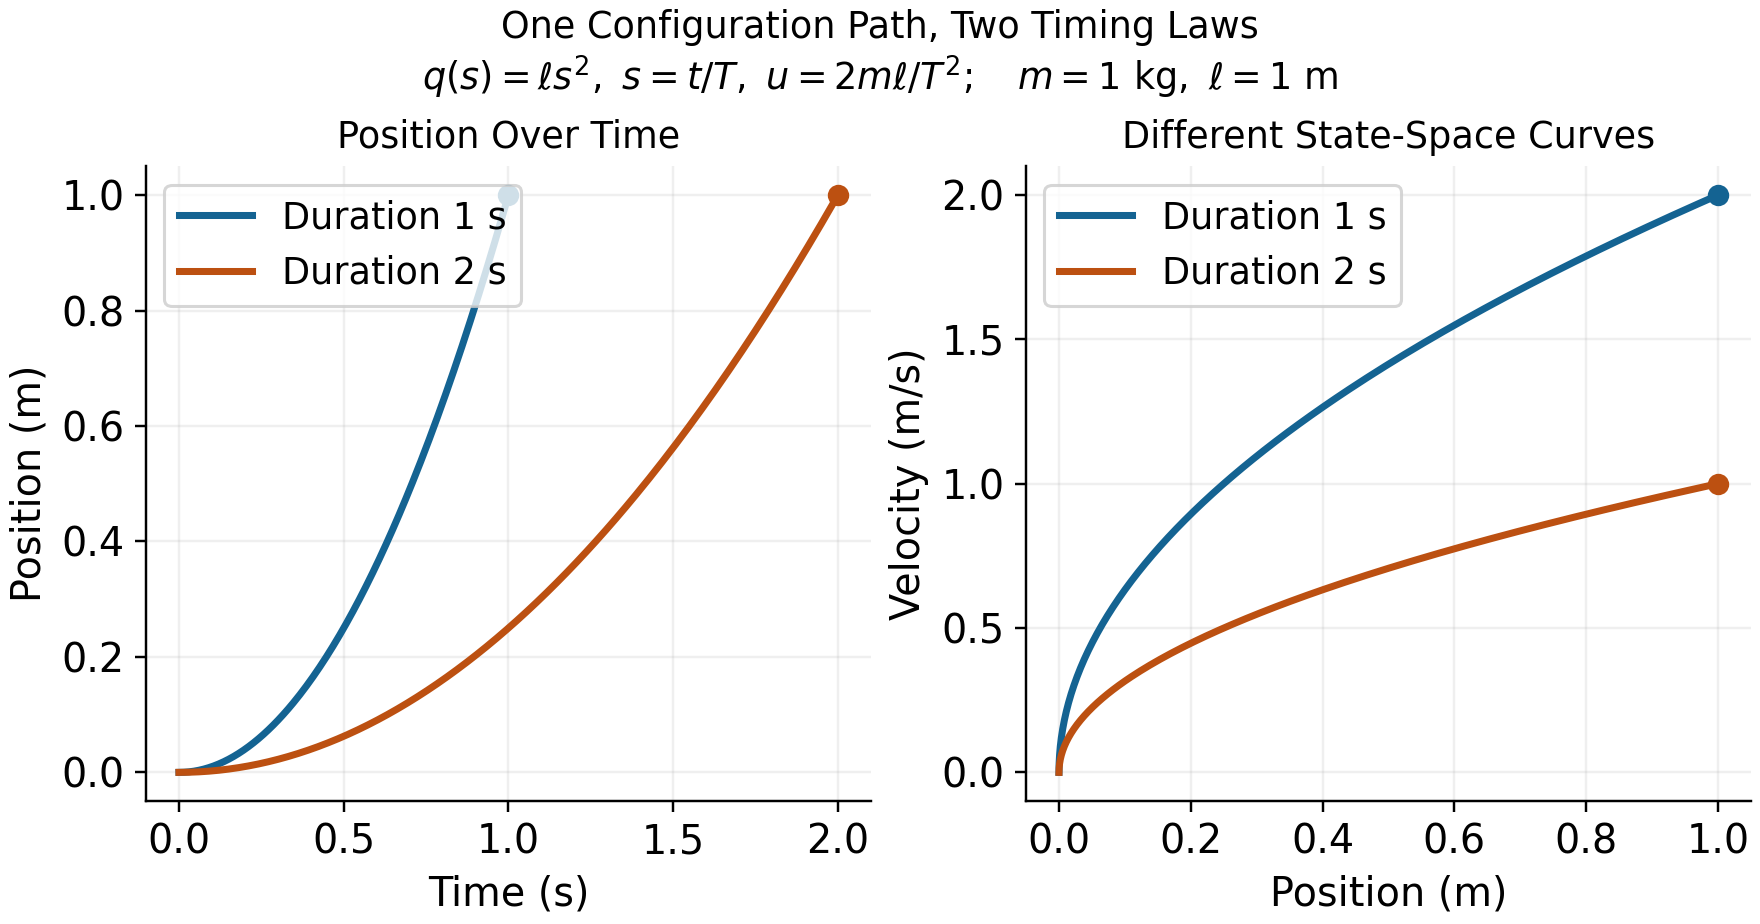
\includegraphics[width=\linewidth]{../The_Geometry_of_Motion/figures/motion_path_timing.png}
\caption{One Configuration Path, Two Timing Laws, and Different State Trajectories. Curves End at the Same Position With Different Velocities.}
\label{fig:motion_path_timing}
\end{figure}

The example uses a prescribed clock-based phase. Estimating phase from the
configuration itself needs care near the stationary start, where $q_d'(0)=0$.
In a swing, a coordinate that reverses at the top of the backswing cannot serve
as a globally increasing phase through that reversal without a different
construction. A useful phase must be defined on the intended interval, be
observable from the chosen state or measurements, and have the required
regularity and progress properties.

\section{Choose a Meaningful Metric and Phase}

A raw norm of position and velocity coordinates mixes different units. Even
among positions, changing metres to centimetres changes an unweighted norm.
One local choice is
\begin{equation}
 \|e\|_W^2=e^TWe,\qquad W=W^T\succ0,
 \label{eq:motion_metric}
\end{equation}
with weights and scales declared according to the desired interpretation.
Under an invertible linear coordinate change $\widetilde e=Se$, the same
quantity uses $\widetilde W=S^{-T}WS^{-1}$. Keeping $W$ unchanged while changing
units generally changes the specification. A physically motivated metric or
scaled output error can be useful, but neither is automatically a clinical
risk measure or an empirical measure of human effort.

On a configuration manifold, subtraction is a local coordinate operation;
rotations, for example, need compatible charts or a chosen local logarithmic
error. The mass matrix defines a kinetic-energy metric on configuration
velocities, not by itself a unique distance on the entire augmented state
including angles, velocities, activation, and other quantities.

For an embedded regular reference curve $\gamma(s)$ in a scaled state chart,
one possible local phase is
\begin{equation}
 s_*(x)\in\arg\min_s\frac12(x-\gamma(s))^TW(x-\gamma(s)).
 \label{eq:motion_projection_phase}
\end{equation}
At an interior minimizer with constant $W$,
\begin{equation}
 \gamma'(s_*)^TW(x-\gamma(s_*))=0.
 \label{eq:motion_phase_orthogonality}
\end{equation}
A sufficiently small tubular neighborhood of a suitably regular embedded curve
can make the projection unique and smooth. That conclusion is local. At the
center of a circle every point on the circle is equally close; self-intersections,
nearby branches, zero tangents, or a finite arc's endpoints can invalidate the
assumed phase chart. A constrained endpoint minimizer need not satisfy the
interior orthogonality equation.

Transverse coordinates need not use nearest-point orthogonality, but must form
valid local coordinates together with phase. If the state dimension is $d$,
there are locally $d-1$ transverse coordinates around a regular one-dimensional
curve. This coordinate count is different from the number of actuators and
from the dimension of a task-equivalent set.

\section{Stability, Attraction, and Finite Motion}

Lyapunov stability means sufficiently small initial errors remain small over
the stated time domain. It does not by itself mean convergence. Asymptotic
stability adds attraction as time tends to infinity. Exponential stability adds
a quantitative decay bound with specified constants. These distinctions apply
to equilibria and have corresponding trajectory and orbital formulations; see
\href{https://underactuated.mit.edu/lyapunov.html}{the MIT Lyapunov analysis notes}.

For a periodic orbit of an autonomous closed-loop system, orbital stability
allows phase displacement while controlling distance to the orbit. A nearby
solution can converge to the orbit without converging to the same clock phase
as a nominal solution. This is useful for periodic motions when phase locking
is not the objective. It is not a general license to change the physical speed
along a prescribed position-velocity curve.

A golf swing studied only up to an impact event is a finite-duration motion.
Its appropriate claims may concern bounded deviation, successful event arrival,
and delivered output tolerances. An infinite-time attraction statement needs
a defined continuation, such as a periodic task or a subsequent stabilization
phase. A finite reference arc is not an invariant orbit once the motion leaves
its endpoint. Bounds on a finite interval should not be renamed asymptotic
stability without that missing structure.

For example, $\dot e=e$ gives $e(t)=e(0)e^t$. On a fixed interval $[0,T]$,
choosing $|e(0)|<\varepsilon e^{-T}$ keeps $|e(t)|<\varepsilon$. This finite-time
bound holds even though errors amplify and the origin is unstable on the
infinite time axis. A useful swing robustness result should therefore report
the permitted initial/measurement uncertainty, the amplification or decay,
the time or event interval, and the terminal output bound.

Orbital analysis still uses Lyapunov functions. For an explicit example,
consider $\dot x_1=x_2$, $\dot x_2=-x_1+u$. The unit circle is a nominal orbit
with $u_d=0$. Put $r^2=x_1^2+x_2^2$ and choose
\begin{equation}
 u=kx_2(1-r^2),\qquad
 V=\tfrac14(r^2-1)^2,\qquad
 \dot V=-k x_2^2(r^2-1)^2\leq0,
 \quad k>0.
 \label{eq:motion_orbit_example}
\end{equation}
On a sufficiently small compact annulus around the unit circle, the largest
invariant subset of $\dot V=0$ is the circle itself. Points with $x_2=0$ away
from the circle do not remain there, since $\dot x_2=-x_1\ne0$; the origin is
excluded by the annulus. Lyapunov and invariance arguments then establish local
orbital attraction and stability. They do not establish phase locking or global
attraction from the origin. The
\href{https://underactuated.mit.edu/limit_cycles.html}{MIT limit-cycle treatment}
and \href{https://arxiv.org/abs/1010.2241}{Manchester's transverse-dynamics analysis}
provide the broader framework.

\section{Verifying a Motion Tube}

A time-varying tube can be defined by
\begin{equation}
 \mathcal T(t)=\{x:V(x,t)\leq\rho(t)\}.
 \label{eq:motion_tube}
\end{equation}
For example, $V$ may measure weighted tracking error. Selecting $\rho(t)$ to
be small near impact expresses a desired tolerance. It does not show that the
closed-loop motion can stay inside the tube. Even $\dot e=0$ leaves a shrinking
tube when initialized on its boundary: constant error cannot fit inside an
arbitrarily decreasing allowed radius.

Suppose the closed-loop dynamics is well posed with admissible inputs,
$V$ and $\rho$ are continuously differentiable, and the tube has a regular
boundary on the domain of interest. For disturbances $d$ in a declared set
$\mathcal D$, a robust inward-boundary condition is
\begin{equation}
 \partial_t V+\nabla_x V^Tf(x,k(x,t),d,t)\leq\dot\rho(t)
 \quad\text{when }V(x,t)=\rho(t),\quad\forall d\in\mathcal D.
 \label{eq:motion_tube_boundary}
\end{equation}
Together with the appropriate regularity and initial membership, this supports
forward invariance over the specified interval. The derivative must include
reference motion and changing metric weights. If $V$ and $\rho$ are indexed
by phase, their derivatives involve the actual $\dot s$; it cannot silently
be replaced by one. Nonsmooth profile corners or hybrid resets need their own
one-sided or transition conditions.

A scalar example makes the effort and disturbance limit explicit. Let
$\dot e=-ke+d$, $|d|\leq\bar d$, and require $|e|\leq r(t)$. On either boundary,
a sufficient condition is
\begin{equation}
 \dot r\geq-kr+\bar d.
 \label{eq:motion_radius_condition}
\end{equation}
For $k=2$, $\bar d=0.1$, and $r(0)=1$ in declared scaled units, the tight
comparison radius is $r(t)=0.05+0.95e^{-2t}$. Constant worst-direction
disturbances attain its two boundaries. The nonzero limiting radius follows
from the disturbance bound and available correction rate. A drawing that
shrinks to zero would not certify this disturbed system.

For an impact specification, also require that every relevant pre-impact
boundary state allowed by the verified tube maps into $\mathcal Y$, and that
the intended event is reached. A phase estimate bounded below by
$\dot s\geq\alpha_{\min}>0$ can supply a progress bound on an appropriate
interval; distance to a path alone cannot. Actuator saturation, sensor delay,
contact feasibility, and uncertainty in the model must be included in the
claimed guarantee. A verified model tube is still a statement about that model
and its declared uncertainty set, not automatic validation on golfers.

\section{Input Rank and Reachability}

For an $n$-coordinate mechanical model with $m<n$ effective inputs, rank limits
instantaneous input acceleration directions. It does not imply that all feasible
states lie on a surface of dimension $2m$. In a state model, drift and input
directions evolve as the system moves; their effect over time can provide
additional reachable directions. The underactuation chapter develops the
associated feasibility and reachability questions.

A concrete counterexample uses two unit masses, one grounded spring, and one
coupling spring, all with unit coefficients. In scaled coordinates,
\begin{equation}
 \ddot q+Kq=bu,\qquad
 K=\begin{pmatrix}2&-1\\-1&1\end{pmatrix},\qquad
 b=\begin{pmatrix}1\\0\end{pmatrix}.
 \label{eq:motion_coupled_springs}
\end{equation}
There is one applied force. With $x=(q_1,q_2,\dot q_1,\dot q_2)^T$,
\begin{equation}
 \dot x=Ax+gu,\qquad
 A=\begin{pmatrix}0&I\\-K&0\end{pmatrix},\qquad
 g=\begin{pmatrix}0\\0\\1\\0\end{pmatrix}.
 \label{eq:motion_spring_state}
\end{equation}
The controllability matrix $[g,Ag,A^2g,A^3g]$ has determinant $-1$ and rank
four. With unconstrained signed inputs, this linear system is controllable in
its full four-dimensional state space. Input limits restrict the size of
reachable sets and time needed; they do not restore the asserted universal
$2m$ dimension bound.

A single trajectory is itself a one-dimensional curve, but the union of
reachable trajectories and the span of a curve's successive derivatives are
different objects. For the same system with $u=0$ and $x(0)=(1,0,0,0)^T$,
the matrix $[Ax,A^2x,A^3x,A^4x]$ at the initial state also has determinant
$-1$. Thus even an unforced example has four independent time derivatives.
At that regular point, smooth arc-length reparameterization preserves their
rank. Actuator count therefore does not cap the number of independent
Frenet-frame directions at $2m$ either.

The useful golf interpretation is more specific. Coupling can transmit and
redistribute the effects of earlier work and present loads. Whether an effective
wrist coordinate is unactuated, weakly actuated, or actively constrained is a
modeling and measurement question. A rapid release does not prove zero wrist
moment, and passive planar dynamics does not guarantee three-dimensional face
squaring. Force, joint moment, mechanical power, and muscle activation must be
kept distinct when testing such hypotheses.

\section{Reliability and Performance}

A path error, a delivery error, and a ball-dispersion measure are different
costs. Choose the one that represents the study, then state how the others
enter the model. Both regulation and trajectory problems can use cost
functionals over an entire history; neither is restricted to a single
instantaneous error value.

For a specified stochastic model and admissible policy $\pi$, one possible
criterion is
\begin{equation}
 \begin{aligned}
 J_\pi&=\phi(y_e)+\int_0^{t_e}\ell(x(t),u(t))\,dt,\\
 \min_\pi\quad&\mathbb E[J_\pi]+\lambda\operatorname{Var}(J_\pi),
 \qquad\lambda\geq0.
 \end{aligned}
 \label{eq:motion_risk_objective}
\end{equation}
The cost and its units, disturbance distribution, event definition, and
constraint handling must be declared. The variance weight has corresponding
units; it expresses a design preference rather than a universal biological
constant. A low variance can accompany a consistently poor mean outcome, so
repeatability alone is not sufficient. Expected cost, tail risk, target-set
probability, and worst-case guarantees answer different questions.
If the intended event is not reached by an allowed horizon, define a failure
cost or constraint; silently discarding those trials changes the question.

A candidate policy may use feedback, a learned reference, or both. Comparing
policies requires recomputing the motion, loads, event time, and output in each
branch. Reusing a measured state or reaction history after the intervention
changes the trajectory can invalidate the comparison. Experimental perturbations
and held-out predictions can test a model; fitting one observed motion does not
establish that the nervous system optimized the proposed criterion.

A practical golf investigation can proceed as follows:
\begin{enumerate}
\item Define the delivered output, its tolerance, and the ball/contact model
      used to connect that output to performance.
\item Declare the mechanical boundary, contact modes, state variables, input
      meaning, parameter uncertainty, and available measurements.
\item Construct compatible nominal states and inputs. Check closure, timing,
      actuator limits, work, and contact feasibility before optimizing a path.
\item Model disturbances and measurement/actuation delays. Compare finite-time
      or event-based output sensitivity and verify any proposed tube condition.
\item Test predictions on independent swings or perturbations, including
      uncertainty in event timing and the inferred loads.
\item Separate demonstrated mechanical identities, validated predictions,
      physiological interpretations, and proposed coaching or design hypotheses.
\end{enumerate}

This is the role of the subsequent chapters: curve geometry describes motion;
configuration manifolds describe compatible coordinates; transverse analysis
and underactuation constrain candidate designs; optimization and robustness
analysis evaluate them; learning and experiments test how well they transfer.
The later golf case study is a modeling proposal unless supported by a complete
specified model, reproducible results, and validation data. The framework's
value comes from making the links testable.

\section{Chapter Exercises}

\begin{enumerate}
\item Specify an impact-event output set that distinguishes clubhead speed,
      face orientation, and impact location. Explain why a terminal target
      does not require stopping there.
\item Derive the error dynamics for the scalar tracking example, then impose
      an input bound and identify where the proposed law becomes infeasible.
\item Reproduce the one-mass timing example. Compare endpoint velocity, input,
      work, and the phase-plane curves for $T=1$ and $T=2$ seconds.
\item For a prescribed pair $(q_d(s),v_d(s))$, derive the compatibility condition
      on $\dot s$ and give an example where arbitrary retiming fails.
\item Rescale a position coordinate from metres to centimetres. Transport the
      error metric and verify that the weighted distance remains unchanged.
\item Show why nearest-point phase is not unique at a circle's center and why
      a finite arc's endpoint needs a separate projection condition.
\item Derive the scalar robust-radius condition and integrate its two
      worst-direction disturbance cases. Explain the nonzero limiting radius.
\item Verify both rank-four matrices in the spring example. Distinguish
      actuator rank, reachable-set dimension, and a trajectory's derivative span.
\item Verify the orbital Lyapunov derivative and the invariant-set argument.
      Explain why this does not prove phase locking or global convergence.
\item Formulate two different reliability objectives for a golf study. State
      what data would distinguish their predictions and what remains unidentifiable.
\end{enumerate}

\chapter{Curves in State Space}
\label{ch:curves_in_state_space}

\section{What a Curve Describes}

A golf swing has several useful geometric descriptions. The clubhead traces a
curve in three-dimensional physical space. The joint configurations trace a
curve in configuration space. Positions, velocities, and any additional
internal states trace a curve in state space. These descriptions answer
different questions. A bend in a plot of joint angle against angular velocity
is not a bend of the clubhead in metres, and its curvature is not a force.

The purpose of this chapter is to make geometry useful without asking it to
supply missing dynamics. We develop arc length, curvature, moving frames,
local transverse coordinates, and timing constraints. We then connect these
tools to physical acceleration, admissible control, and the impact task.
Geometry specifies a motion's shape within a stated space and metric.
Dynamics determines which timed motions and corrections are possible.
Measurements determine whether a proposed model describes an actual swing.

Throughout the Euclidean calculations, the ambient space is $\mathbb R^d$
with a specified inner product. A prime denotes differentiation with respect
to the displayed curve parameter; a dot denotes physical time. A regular
curve has a nonzero first derivative on the interval under discussion.
Configurations are denoted by $q$, full states by $x$, and a physical point
such as the clubhead by $p$. We use $s$ for arc length and $\lambda$ for a
parameter that need not measure distance.

\subsection{Geometry Depends on the Space and Metric}

Euclidean curvature is invariant under regular reparameterization and rigid
changes of Cartesian frame. It is an extrinsic property of the embedded
curve: it measures how the curve bends in its ambient space. Calling this
``intrinsic'' merely because it does not depend on timing confuses two uses
of geometry. A straight segment and a circular arc of the same length have
the same one-dimensional arc-length metric, although their ambient
curvatures differ.

Changing units without transforming the metric changes the calculation.
For a state $x=(q,\dot q)$, a raw sum of squared positions and velocities has
no universal physical meaning. One possible declared convention is
$z=Sx$, where $S$ contains inverse reference scales, followed by Euclidean
geometry in the dimensionless coordinates $z$. Different scales generally
give different curvature signatures. This is a modeling choice to report
and test, not a coordinate-free marker of skill.

For a positive-definite metric $W$, the squared displacement is
$dx^T W dx$. Under $z=Sx$, the same metric has matrix
$\widetilde W=S^{-T}WS^{-1}$. A constant metric can be handled through a
linear change to orthonormal coordinates. With a position-dependent metric,
ordinary second derivatives are not sufficient: curvature uses the
appropriate covariant derivative. The kinetic-energy matrix $M(q)$ defines
a metric on configuration velocities; it is not automatically a metric on
an augmented state containing velocities, activation, and contact variables.

\section{Regular Parameters and Arc Length}

Let $\gamma:I\rightarrow\mathbb R^d$ be a $C^2$ curve, and let
$h(\lambda)=\|\gamma'(\lambda)\|>0$. Its arc-length function and unit tangent are
\begin{equation}\label{eq:arc_length}
 s(\lambda)=\int_{\lambda_0}^{\lambda}h(\mu)\,d\mu,
 \qquad T(\lambda)=\frac{\gamma'(\lambda)}{h(\lambda)}.
\end{equation}
Because $ds/d\lambda=h>0$, the inverse function theorem gives a local regular
arc-length parameter. In that parameter $\|\gamma'(s)\|=1$ and
$T=\gamma'(s)$. Replacing $\lambda$ by a smooth increasing diffeomorphism
changes the rate of traversal while preserving the oriented curve.
A merely increasing function can have zero derivative and need not preserve
regularity at every point.

For example, $(\cos t,\sin t)$ and $(\cos t^2,\sin t^2)$ trace the same circle
on suitable intervals. The second time parameterization has zero velocity
at $t=0$. Arc-length formulas that divide by speed apply for $t>0$; the
circle's geometry can separately be extended through the starting point.
A temporal stop is not by itself a geometric cusp or an infinite curvature.

A reversal is even more informative. In normalized coordinates, the physical path
$p(t)=(t^2,0)$ has zero curvature on either side of $t=0$, while velocity
vanishes and reverses there. The unit tangent defined by time is undefined
at the reversal. The full mechanical state
$x(t)=(t^2,2t)$ has derivative $(2t,2)$ and is regular at the same instant.
Thus the physical point can stop while the state continues moving. There is
no universal conclusion that the top of a backswing is the point of maximum
curvature in any of these spaces.

If a regular configuration path is parameterized by $\lambda$ and traversed
with $\dot\lambda>0$, its chosen-metric speed is
$\dot s=\|q'(\lambda)\|\dot\lambda$. In particular, $\dot\lambda$ is not
Cartesian speed unless the path is parameterized by physical arc length.
This distinction matters when converting a speed limit into a timing law.

\section{Curvature and Physical Acceleration}

For a unit-speed $C^2$ Euclidean curve,
\begin{equation}\label{eq:curvature_def}
 k(s)=\frac{dT}{ds},\qquad \kappa(s)=\|k(s)\|.
\end{equation}
Differentiating $T^TT=1$ gives $T^Tk=0$. Where $\kappa>0$, the principal
normal is $N=k/\kappa$. At a point with zero curvature, $k$ remains defined
but this particular normal does not. Curvature vanishing on an entire
connected regular interval makes $T$ constant and the curve a straight
segment. Vanishing at one point does not: $(t,t^3)$ has zero curvature at
$t=0$ and bends arbitrarily nearby.

For any regular parameter, differentiating the normalized tangent gives
\begin{equation}\label{eq:curvature_general_n}
 \kappa=\frac{\|(I-TT^T)\gamma''\|}{\|\gamma'\|^2}
 =\frac{\sqrt{\|\gamma'\|^2\|\gamma''\|^2-(\gamma'^T\gamma'')^2}}
 {\|\gamma'\|^3}.
\end{equation}
In three dimensions the numerator of the final expression is
$\|\gamma'\times\gamma''\|$. In two dimensions it is the absolute determinant
of the two derivative vectors. There is no need to invent an ordinary cross
product in arbitrary dimension. The projected-acceleration form also avoids
subtracting two large nearly equal squared quantities, although numerical
error can still dominate near zero speed.

\subsection{A Checkable Ellipse}

For $\gamma(\lambda)=(a\cos\lambda,b\sin\lambda)$ with $a>b>0$,
\begin{equation}
 \kappa(\lambda)=\frac{ab}
 {(a^2\sin^2\lambda+b^2\cos^2\lambda)^{3/2}}.
\end{equation}
The major-axis endpoints $(\pm a,0)$, at $\lambda=0,\pi$, have the largest
curvature $a/b^2$. The minor-axis endpoints $(0,\pm b)$ have the smallest
curvature $b/a^2$. With $a=2$ m and $b=1$ m these are $2$ and $0.25$ inverse
metres. Uniformly changing the rate of traversal preserves these values.
Stretching a circle into this ellipse does not preserve curvature.

\subsection{Where the Speed-Squared Law Applies}

Let $p(s)$ now be a physical position in an inertial Cartesian frame, with
$s$ measured in metres, and let $v=\dot s>0$. The chain rule gives
\begin{equation}\label{eq:centripetal}
 \dot p=vT,\qquad \ddot p=\dot vT+v^2k
 =\dot vT+v^2\kappa N\quad(\kappa>0).
\end{equation}
Here $v^2\kappa$ is a physical normal acceleration in m/s$^2$. The identity
is kinematic: it describes the acceleration of the prescribed motion before
assigning which forces produce it.

For a point mass, Newton's law says
\begin{equation}\label{eq:control_demand}
 m\ddot p=F_{\mathrm{act}}+F_{\mathrm{pass}}+F_{\mathrm{external}}
 +F_{\mathrm{reaction}}.
\end{equation}
Only in a model where the actuator supplies the entire resultant force does
$F_{\mathrm{act}}=m(\dot vT+v^2k)$. Gravity, springs, contact, and constraint
reactions can contribute. A $0.2$ kg mass moving at $20$ m/s on a horizontal
circle of radius $1$ m requires $80$ N inward. In an ideal frictionless
circular guide with no tangential resistance, the guide supplies that force
and does zero work because its force is perpendicular to velocity. No
continuous actuator work is needed to maintain the speed in this model.
That calculation does not show that a golfer supplies zero joint moments.
It shows why resultant acceleration and active effort are different
quantities.

A clubhead is a point on a moving, rotating, possibly flexible body rather
than an isolated point mass with all force applied at that point. For a
rigid model with $p=p(q)$,
\begin{equation}
 \dot p=J_p(q)\dot q,\qquad
 \ddot p=J_p(q)\ddot q+\dot J_p(q,\dot q)\dot q.
\end{equation}
The Jacobian-rate term supplies normal acceleration even at constant joint
speed. Segment force and moment balances, distributed mass, hand wrenches,
and any modeled shaft deflection are needed to interpret measured clubhead
acceleration. Multiplying it by total club mass does not generally recover
the hand force.

For a first-order state equation $\dot x=f(x,u,t)$, the analogous curve
identity concerns $\ddot x$, which may include mechanical jerk and internal
state derivatives. When $u$ is differentiable,
\begin{equation}
 \ddot x=f_xf+f_u\dot u+f_t.
\end{equation}
This is not a generic decomposition of $u$ into tangential and normal
forces. The reference condition remains
$f(\gamma(s(t)),u_*(t),t)=\gamma'(s(t))\dot s(t)$, together with input
admissibility. In an autonomous model the final argument is absent.

\section{Moving Frames and Their Limits}

\subsection{An Oriented Three-Dimensional Frame}

For a $C^3$ regular curve in oriented Euclidean three-space with $\kappa>0$,
define $T=dp/ds$, $N=T'/\kappa$, and $B=T\times N$. Then
\begin{equation}\label{eq:frenet_serret}
 \frac{dT}{ds}=\kappa N,\qquad
 \frac{dN}{ds}=-\kappa T+\tau B,\qquad
 \frac{dB}{ds}=-\tau N.
\end{equation}
The signed torsion is
\begin{equation}
 \tau=\frac{\det[p',p'',p''']}{\|p'\times p''\|^2},
\end{equation}
where the primes in this formula may use any regular parameter. Torsion
requires nonzero curvature. A planar regular curve has zero torsion where
the formula is defined; at an inflection the Frenet normal and torsion may
be undefined even when the original curve is smooth.

For the helix $p(\lambda)=(a\cos\lambda,a\sin\lambda,b\lambda)$ with $a>0$,
\begin{equation}
 \kappa=\frac{a}{a^2+b^2},\qquad \tau=\frac{b}{a^2+b^2}.
\end{equation}
Changing the sign of $b$ reflects the helix and changes the sign of torsion.
Proper rotations and translations preserve both. Blindly applying
Gram--Schmidt to all three derivatives chooses the final vector from the
third derivative's residual; it can produce $-B$ when torsion is negative.
That convention cannot simultaneously be identified with the oriented
binormal $T\times N$ without tracking the sign.

In this physical three-dimensional setting, torsion measures rotation of the
osculating plane per unit distance. Torsion of a normalized state-space curve
has a different ambient space and interpretation. It is not a direct measure
of anatomical rotation or of how a golfer should change the swing plane.

\subsection{Higher Dimensions and Regular Normal Frames}

With sufficient smoothness and independent successive derivatives,
Gram--Schmidt constructs an orthonormal basis for the successive osculating
spaces of a curve in $\mathbb R^d$. A full oriented Frenet frame can be chosen
by orthogonalizing the first $d-1$ independent derivatives and completing the
last vector with a fixed ambient orientation. Its equations have the form
\begin{equation}
 e_i'=-\kappa_{i-1}e_{i-1}+\kappa_i e_{i+1},
 \qquad \kappa_0=\kappa_d=0.
\end{equation}
The first $d-2$ curvatures are positive under the required independence
conditions; the final oriented curvature can have either sign or vanish.
Alternatively, a frame made from all $d$ independent derivatives adopts a
different sign convention. State the convention before comparing signatures.
If only a partial frame is constructed, its last derivative need not remain
inside that partial span. A closed lower-dimensional Frenet system needs an
appropriate containing affine subspace and its own regularity assumptions.

There is a simpler option for local control: choose any smooth orthonormal
normal frame $E(s)$, with $d-1$ columns, satisfying
$T^TE=0$ and $E^TE=I$. Define
\begin{equation}
 c=E^TT',\qquad \Omega=E^TE',\qquad
 T'=Ec,\qquad E'=-Tc^T+E\Omega.
\end{equation}
Differentiating $E^TE=I$ shows that $\Omega$ is skew-symmetric. A parallel
normal frame, often called a Bishop frame, chooses $\Omega=0$ locally along
an interval. It continues through zero-curvature points of a regular curve
where the principal Frenet normal fails. Such a frame still requires an
initial normal orientation; a periodic curve can have a nontrivial change
of normal orientation after one circuit.

The number of normal coordinates is $d-1$, not the actuator count. The
one-input spring example in the previous chapter has four independent
unforced trajectory derivatives at its specified initial state. A single
trajectory is one-dimensional, its osculating span can be larger, and the
union of reachable trajectories is another object again.

\section{Shape Reconstruction and Its Limits}

For continuously differentiable $\kappa(s)>0$ and continuous signed
$\tau(s)$ on an interval,
the three-dimensional Frenet equations, together with $p'=T$, reconstruct a
unit-speed curve once its initial point and oriented frame are specified.
Existence and uniqueness follow from the frame's linear differential
equation and integration of $T$. Without the initial point and frame, the
curve is determined up to a proper rigid motion. Analogous statements in
higher dimensions require a complete consistent curvature list and frame
convention; an arbitrary truncated signature is insufficient.

Congruence is not equality relative to the golf ball. Translating or rotating
a clubhead path can make it miss the ball while preserving its curvature and
torsion. A rigid rotation of normalized position-velocity coordinates need
not even correspond to a physically allowed state transformation. Gravity,
contact, anatomy, and the target frame further restrict useful symmetries.
Neither shape reconstruction nor a similar curvature signature establishes
equal timing, forces, face orientation, or performance.

Where $\kappa>0$, the osculating circle has center $p+N/\kappa$ and radius
$1/\kappa$. It matches local position, tangent, and curvature; the tangent
line and osculating plane supply lower-order geometric descriptions. An
osculating sphere in three dimensions needs additional conditions. Writing
$\rho=1/\kappa$, when $\tau\ne0$ its center is
$p+\rho N+(\rho'/\tau)B$. This follows by requiring successive derivatives
of squared distance to a fixed center to vanish through third order. At
zero torsion the construction may fail or be nonunique, depending on
$\rho'$. It is not an unconditional approximation for every high-dimensional
state curve.

\section{Feasible Timing and Available Forces}

For a chosen configuration path $q=q(\lambda)$,
\begin{equation}
 \dot q=q'\dot\lambda,\qquad
 \ddot q=q''\dot\lambda^2+q'\ddot\lambda.
\end{equation}
Substitution into mechanical dynamics gives the required generalized load:
\begin{equation}\label{eq:curve_path_dynamics}
 M(q)(q'\ddot\lambda+q''\dot\lambda^2)+h(q,q'\dot\lambda)
 =B(q)u+Q_{\mathrm{pass}}+Q_{\mathrm{external}}+J_c^T\eta.
\end{equation}
Here $h$ contains the declared velocity and potential terms, and passive
terms must not be counted twice. The path must satisfy configuration
constraints; its derivatives must satisfy their velocity and acceleration
conditions. Contact reactions $\eta$, friction, actuator bounds, activation
dynamics, and any force-rate limits constrain feasible timing. For an
underactuated system, not every desired generalized load lies in the input
image even if every motor is individually below its limit.

For a fully actuated model, each torque bound can become an inequality in
$\lambda$, $\dot\lambda$, and $\ddot\lambda$. This is the basis of
path-constrained time scaling. It is more informative than assigning a
single curvature cost because it retains gravity, inertia, coupling, and
the available input directions. The configuration path and timing can be
optimized in stages, but their feasibility constraints remain coupled.
Retiming also changes the corresponding full state curve, as shown in the
previous chapter.

A simple point-mass model gives a useful limited speed bound. Suppose the
actuator supplies the entire force, with $\|F\|\le F_{\max}$, and there are
no other forces. On a physical arc-length path,
\begin{equation}
 \dot v^2+(\kappa v^2)^2\le(F_{\max}/m)^2.
\end{equation}
Thus $v\le\sqrt{F_{\max}/(m\kappa)}$ is necessary when $\kappa>0$, but leaves
no force for tangential acceleration at equality. For $m=2$ kg,
$F_{\max}=10$ N, $\kappa=0.5$ m$^{-1}$, and $v=3$ m/s, the normal
acceleration is $4.5$ m/s$^2$ and the remaining tangential bound is
$\sqrt{25-4.5^2}=\sqrt{4.75}$ m/s$^2$. If a guide supplies normal reaction,
the actuator's feasible set is different.

At zero curvature this particular normal-acceleration bound supplies no
speed ceiling. Tangential acceleration, initial and terminal conditions,
velocity limits, power, and the next bend can still limit speed. A
minimum-time exercise based only on normal acceleration can therefore lack
an attained smooth solution or a physically meaningful optimum. Prescribe
the full bounds and endpoint conditions before claiming an optimal law.

\section{Local Phase and Transverse Dynamics}

\subsection{Coordinates in a Tubular Neighborhood}

Let $\gamma(s)$ be a regular embedded unit-speed state curve in a chosen
Euclidean metric, and choose the smooth normal frame $E(s)$ above. In a
sufficiently small neighborhood of an interior segment, write
\begin{equation}\label{eq:frenet_coords}
 x=\gamma(s)+E(s)\xi.
\end{equation}
Nearest-point phase satisfies $T^T(x-\gamma)=0$ there. Local uniqueness
requires more than this stationary equation: the curve must not intersect
itself in the neighborhood, and the coordinate Jacobian must be invertible.
The scalar factor $1-c^T\xi$ in that Jacobian must be nonzero. A smaller
neighborhood may be needed to exclude other closest points. For a circle,
the center has many nearest points and the inward normal coordinates become
singular there. Endpoints require one-sided treatment. A regular local
normal frame does not turn all nearby states into a single global chart.

Let the smooth autonomous dynamics be $\dot x=f(x,u)$ and suppose a feasible
nominal input satisfies
$f(\gamma(s),u_*(s))=v_*(s)T(s)$ with $v_*>0$. Differentiate the coordinate
map and project onto $T$ and $E$:
\begin{equation}\label{eq:curve_exact_transverse}
 \dot s=\frac{T^Tf(x,u)}{1-c^T\xi},\qquad
 \dot\xi=E^Tf(x,u)-\Omega\xi\dot s.
\end{equation}
These equations retain both the phase denominator and the normal-frame
transport. They are coordinate-rate equations; the word ``force'' should
not be assigned to every transport term in a first-order state model.

With $u=u_*(s)+\delta u$, the transverse linearization at $\xi=0$ is
\begin{equation}\label{eq:transverse_lin}
 \dot\xi=A_\perp(s)\xi+B_\perp(s)\delta u
 +O(\|(\xi,\delta u)\|^2),
\end{equation}
where
\begin{equation}
 A_\perp=E^Tf_x(\gamma,u_*)E-v_*\Omega,
 \qquad B_\perp=E^Tf_u(\gamma,u_*).
\end{equation}
All partial derivatives here hold $s$ fixed; nominal phase evolves by
$\dot s=v_*(s)$. For explicitly time-dependent dynamics, include the time
state or derive the corresponding time-dependent coordinate map. A
feedback depending on an independently prescribed clock is also a different
problem from the phase-indexed law assumed here.

There is no universal correction of the form speed squared times a curvature
matrix subtracted from the original Jacobian. Curvature enters the phase
map and chosen frame; transverse stability depends on the actual vector
field, its derivatives, input directions, feedback, and regularity.
Changing the normal basis changes the coordinate matrices consistently,
without changing physical attraction of the orbit.

\subsection{The Same Circle With Opposite Stability}

In a neighborhood of $r=R>0$, consider the planar systems
\begin{equation}
 \dot r=a(r-R),\qquad \dot\theta=\omega>0.
\end{equation}
Every value of $a$ has exactly the same nominal circle, curvature $1/R$,
speed $R\omega$, and nominal time parameterization. Yet radial error evolves
as $e(t)=e(0)e^{at}$: $a<0$ attracts, $a>0$ repels, and $a=0$ is neutral.
Curvature and nominal speed cannot distinguish these cases. The figure uses
$R=2$ and $\omega=1.3$, with initial radii $1.8$ and $2.2$, over four model
time units. Its radial growth rates are $a=-0.3$ and $a=0.3$.

\begin{figure}[htbp]
\centering
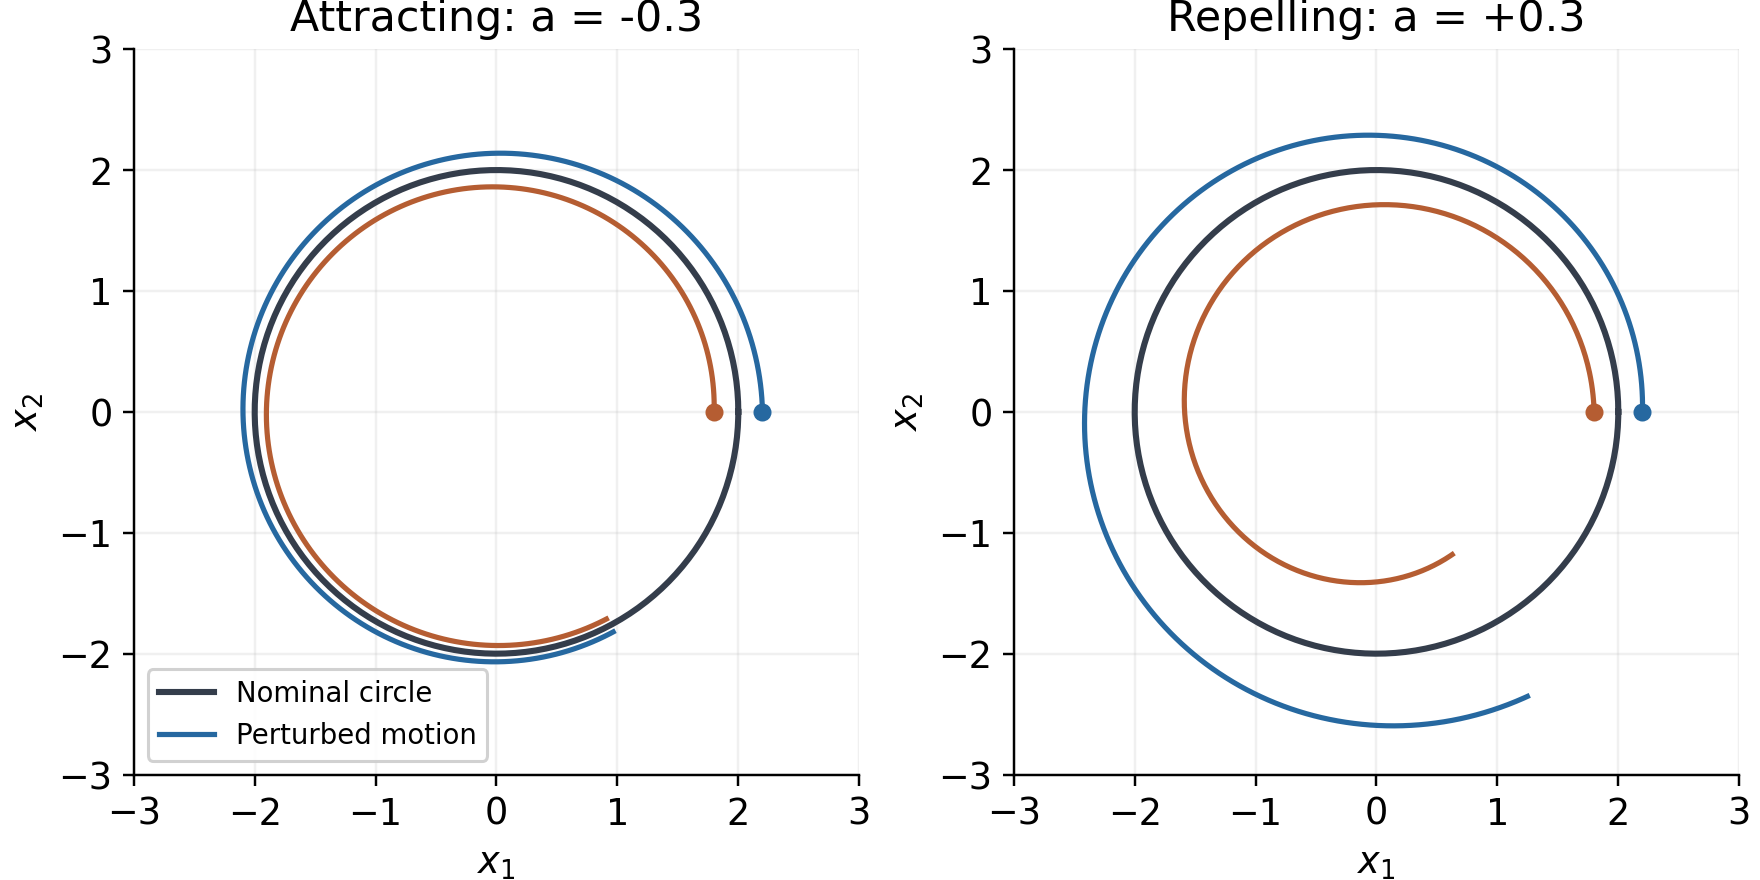
\includegraphics[width=\textwidth]{../The_Geometry_of_Motion/figures/curve_stability_comparison.png}
\caption{The Same Nominal Circle With Opposite Transverse Stability}
\label{fig:curve_stability_comparison}
\end{figure}

Using the inward normal coordinate $\xi=R-r$ and arc length $s=R\theta$
gives $\dot\xi=a\xi$ and $\dot s=R\omega$. The exact phase formula agrees:
$T^Tf=\omega(R-\xi)$ and $1-c^T\xi=1-\xi/R$. Their ratio is $R\omega$.
This checks the denominator as well as the transverse linearization. A
geometric tube around the circle becomes a verified invariant tube only
when the actual transverse dynamics and disturbances satisfy its boundary
condition.

\section{Curvature and Reachability Are Different}

For a control-affine system, instantaneous input directions, reachable sets,
and the derivatives of one trajectory are distinct. Lie brackets describe
noncommuting flows. With the convention
$[g_i,g_j]=Dg_j\,g_i-Dg_i\,g_j$, the bracket can expose a displacement
direction generated by suitable short sequences of controls. The
Chow--Rashevskii result concerns bracket-generating driftless systems under
appropriate smoothness and reversible control assumptions. The orbit
theorem describes the geometry of orbits of vector fields and is not the
same theorem. Allowing forward and backward field flows to define an orbit
does not automatically describe forward-time reachability with drift,
unilateral contact, or bounded controls.

A curved path need not use nonzero brackets at all. For the planar integrator
$\dot x=u$, the two constant input fields commute. The control
$u(t)=(-\sin t,\cos t)$ traces the unit circle from $(1,0)$ with curvature
one. Its acceleration comes from changing the input, while every bracket of
the constant input fields is zero. Conversely, a system can have useful
bracket directions without expressing them as a large curvature along one
recorded trajectory. High curvature does not identify a commutator, a neural
synergy, or an underactuated strategy.

\section{Using Geometry in a Golf Investigation}

A useful investigation keeps the chain of interpretation explicit:
measurement, geometric description, feasible mechanics, uncertainty, and
task outcome. Consider the following protocol.

\begin{enumerate}
\item Choose the object and frame. A clubhead point, shaft orientation,
   joint configuration, and complete state are different data products.
   Use a target-fixed physical frame for ball delivery. State how angles,
   rotations, velocities, and internal states are represented.
\item Report units and metric scales. For a state signature, repeat the
   calculation under plausible scaling choices. For three-dimensional
   clubhead curvature, use physical positions in consistent length units.
\item Fit derivatives with an explicit measurement model. Differentiation
   amplifies noise; torsion requires a third derivative and is especially
   fragile near small curvature or speed. Report sampling, smoothing,
   uncertainty, and sensitivity to filtering. Do not divide by near-zero
   denominators and then interpret numerical spikes as swing phases.
\item Align trials using a declared event or phase convention. Compare both
   geometric shape and timing; report where a reference curve's nearest
   projection becomes ambiguous. Treat impact and contact changes using
   one-sided smooth segments or a hybrid model.
\item Compute physical acceleration and mechanical load with the appropriate
   Jacobians, inertias, external loads, and constraints. Distinguish net
   joint moments from muscle recruitment and resultant force from work.
   Validate these quantities against independent measurements where possible.
\item Evaluate pre-impact speed, face orientation, path direction, strike
   location, and relevant ball outcomes with uncertainty. Test whether a
   geometric feature predicts outcomes beyond simpler measured variables
   on held-out trials. A correlation does not identify the control policy.
\item Test interventions in a declared forward model and then seek empirical
   validation. Altering timing can change speed-dependent loads and contact
   feasibility; altering a path can change moment arms and the impact frame.
   Recompute the complete trajectory rather than attaching a new conclusion
   to an unchanged force history.
\end{enumerate}

The hypothesis that golfers exploit passive coupling remains worth testing.
The geometric tools can identify repeatable patterns and organize model
comparisons. They cannot by themselves establish that a particular pause,
release, curvature peak, or low-dimensional signature is optimal, automatic,
or a consequence of a particular neural strategy. Those arguments require
mechanics and evidence at the next links in the chain.

\section{Further Reading}

The geometric conventions can be checked against
\href{https://www.math.ucla.edu/~petersen/DGnotes.pdf}{Petersen's Classical
Differential Geometry}, especially its curve, Frenet, and parallel-frame
treatments. Path-constrained timing and torque bounds are developed in
\href{https://modernrobotics.northwestern.edu/nu-gm-book-resource/9-4-time-optimal-time-scaling-part-1-of-3/}{Lynch and Park's Modern Robotics}.
For transverse dynamics and orbital stabilization, see
\href{https://arxiv.org/abs/1010.2241}{Manchester's Transverse Dynamics and
Regions of Stability for Nonlinear Hybrid Limit Cycles}. These are
mathematical and robotics references; they do not validate the golf-specific
hypotheses in this chapter.

\section{Exercises}

\begin{enumerate}[itemsep=2pt,parsep=0pt]
\item For $(t,t^3)$, derive the curvature and show why its zero value at the
   origin does not imply a straight neighborhood. Contrast this with the
   stopped physical path $(t^2,0)$ and its regular position-velocity state.
\item Derive the ellipse formula and identify its major- and minor-axis
   endpoint curvatures. Verify invariance under $t\mapsto 2t$ and explain
   why stretching only one coordinate changes the Euclidean answer.
\item Compute curvature and signed torsion for $(t,t^2,t^3)$ at $t=0$ and
   $t=1$. Explain what extra mechanical assumptions are needed to compare
   actuator effort along the two portions of the curve.
\item For the helix $(2\cos t,2\sin t,t)$, calculate $T,N,B,\kappa,\tau$.
   Reflect its third coordinate and track the sign of the oriented torsion.
\item Derive the exact normal-coordinate equations by projecting the
   derivative of $x=\gamma(s)+E(s)\xi$. Identify the coordinate singularity
   for a circle and verify the radial stability counterexample.
\item A $2$ kg point mass is driven solely by a force of norm at most
   $10$ N. Find the available tangential acceleration at speed $3$ m/s on a
   radius-$2$ m circle. Repeat the interpretation when an ideal guide
   supplies all normal reaction.
\item Let $p(\lambda)=\ell(\lambda,\sin(\pi\lambda),0)$ for
   $0\le\lambda\le2$, where $\ell=1$ m. Derive the curvature and the
   conversion from $\dot\lambda$ to physical speed. Formulate a timing
   optimization with a total-acceleration bound, a finite speed bound, and
   zero initial and terminal speeds; do not assume that a bound on normal
   acceleration alone specifies a smooth minimum-time solution.
\item Starting with a declared double-pendulum model, generate a smooth
   swing-like segment and compare configuration, physical clubhead, and
   normalized state curvature. Repeat under different state scales and
   sampling noise. Report which features remain stable and which do not.
\item Construct two congruent physical paths with different positions
   relative to a fixed ball. Explain why their curvature signatures agree
   while their impact outcomes differ.
\item For a measured or simulated swing, propose one geometric hypothesis,
   its mechanical interpretation, a competing explanation, an independent
   validation measurement, and a criterion that could falsify it.
\end{enumerate}

\chapter{Configuration Manifolds}
\label{ch:configuration_manifolds}

\section{Describe the System Before Choosing Coordinates}

A club has a position and an orientation. An elbow angle describes a relative
configuration, while clubface orientation describes an output of the entire
kinematic chain. Angular velocity adds information that a configuration does
not contain. These distinctions matter when comparing swings: a small change
in a joint coordinate can accompany a large change in an impact outcome, and
a large coordinate jump can occur while the physical motion remains smooth.
Geometry helps us distinguish these possibilities. It does not determine which
motion a golfer should make without a mechanical model and an outcome criterion.

Coordinates are measurements expressed as numbers. They are legitimate local
descriptions, not false versions of the physical system. A useful model states
what configurations are identified, what constraints apply, and where its
coordinates remain valid. Some mechanical configuration spaces are Euclidean;
others require multiple charts or a constrained representation. The relevant
question is whether the chosen description covers the motion being analyzed
without ambiguity that the analysis fails to handle.

An ideal revolute joint with unlimited rotation has configuration space $S^1$
when a full turn restores every modeled property. If cable winding, accumulated
twist, or another internal variable distinguishes successive turns, that angle
alone is not a complete configuration. A joint restricted between two stops
instead has an interval of admissible angles. Its interior admits a single
real coordinate; the endpoints require a boundary or contact model. These
models answer different questions and should not be interchanged silently.

A smooth $n$-dimensional manifold is a Hausdorff, second-countable space locally
described by open subsets of $\mathbb R^n$, with smooth invertible transitions
between overlapping coordinate charts. This definition covers $\mathbb R^n$
itself. A chart need not cover the entire space, but some manifolds do admit one
global chart. A circle does not admit a single nonsingular real coordinate
with all its identifications preserved. Embedding it as $(\cos\theta,\sin\theta)$
uses two numbers subject to one constraint rather than creating a second
degree of freedom. Boundaries, corners, changing contact modes, and singular
constraint sets require qualifications beyond an ordinary smooth manifold.

\subsection{Configurations, Directions, and Task Outputs}

A spherical pendulum whose only configuration is the direction of a rigid rod
has space $S^2$. An unconstrained rigid-body orientation has space $SO(3)$,
which also records rotation about the rod's axis. A two-axis universal joint
consists of ordered revolute joints. With ideal unlimited independent angles,
its joint configuration space is $S^1\times S^1$, not automatically $S^2$.
Its pointing-direction output may cover a sphere with repeated or singular
representations. Joint limits, interference, or closure can restrict that
space. Counting two degrees of freedom does not identify its topology.

An open ideal chain with two spherical joints and three revolute joints has
the nine-dimensional configuration space
\begin{equation}\label{eq:golf_config}
 Q_0=SO(3)\times SO(3)\times(S^1)^3,\qquad \dim Q_0=9.
\end{equation}
This can be a teaching model of torso, shoulder, elbow, and wrist motion.
It is not an anatomical assertion that those joints rotate without limits,
nor a complete two-handed golfer. A real model must state its pelvis/ground
attachment, joint axes, ranges, hand contacts, and whether shaft flexibility
or grip compliance is represented. Shoulder translation and distributed
spinal motion may matter for the chosen question.

Smooth holonomic constraints $\Phi(q)=0$ with independent Jacobian rows define
a local submanifold of dimension $n-\operatorname{rank}D\Phi$. Velocities then
satisfy $D\Phi(q)\dot q=0$. At changing rank, this dimension argument needs
reassessment. Unilateral contact also has inequalities and mode transitions.
A velocity constraint need not integrate to a configuration constraint.
Consequently, a closed chain cannot be analyzed by adding nominal joint
degrees of freedom and ignoring closure. Nor does configuration dimension
give the number of independently identifiable hand forces or muscle inputs.

The clubhead position $p(q)$ and face orientation $R_c(q)$ are task maps out
of this configuration space. Their derivatives can lose rank even when the
configuration coordinates are regular. Conversely, singular coordinates can
be replaced without changing the rank of a physical task map. Keeping these
two questions separate is essential when interpreting a large wrist-angle
change or a poorly conditioned inverse calculation.

\section{Velocities, Forces, and Mechanical State}

A tangent vector at $q$ describes an infinitesimal configuration change. In
coordinates it has components $v^i$, and a mechanical velocity is one such
vector. The tangent bundle $TQ$ collects all pairs $(q,v)$. For a regular
second-order mechanical model with no additional internal state, it is a
natural state space of dimension $2n$. Muscle activation, viscoelastic memory,
flexible modes, controller state, and contact mode can require an augmented
state. A configuration path alone does not determine any of these quantities.

A generalized force is a covector $F\in T_q^*Q$: it acts on a virtual
displacement to give virtual work, and on velocity to give power. In coordinates,
\begin{equation}\label{eq:manifold_force_power}
 \delta W=F_i\,\delta q^i,\qquad P=F_i\dot q^i.
\end{equation}
Repeated indices are summed here. A torque represented by a three-vector in
a chosen orthonormal frame uses an identification between vectors and
covectors; this convenience should not obscure the dual role of force.
Mass and inertia provide a different identification in generalized coordinates.

Let new coordinates be $z=\psi(q)$ with invertible Jacobian $A=D\psi$.
Velocity components transform as $v_z=A v_q$, whereas force components
transform as $F_z=A^{-T}F_q$. Therefore $F_z^Tv_z=F_q^Tv_q$: physical power
does not depend on the coordinate units or chart. Transforming both with $A$
would generally destroy this equality. This is a direct diagnostic for
incorrect unit scaling in a swing model.

For a positive-definite mass matrix $M(q)$, kinetic energy is
\begin{equation}\label{eq:manifold_kinetic_metric}
 T(q,v)=\tfrac12v^TM(q)v,\qquad
 M_z=A^{-T}M_qA^{-1}.
\end{equation}
It defines an inner product on configuration tangent vectors. Redundant
coordinates, massless idealizations, or uneliminated constraints can instead
give a singular matrix; then a positive-definite metric must be justified on
the appropriate reduced tangent space. The configuration mass matrix is not
automatically a metric on the augmented position/velocity/activation state.

\section{Rotations and Three Different Singularities}

We use active rotation matrices $R\in SO(3)$ mapping body components into
world components. Thus $R^TR=I$ and $\det R=1$. Body angular velocity $\omega$
and world angular velocity $\omega_w$ satisfy
\begin{equation}\label{eq:manifold_rotation_kinematics}
 \dot R=R\widehat\omega=\widehat{\omega_w}R,\qquad
 \omega_w=R\omega,\qquad \widehat a\,b=a\times b.
\end{equation}
Nine matrix entries describe three rotational degrees of freedom subject to
constraints. A numerical integrator must preserve or appropriately restore
these constraints. This representation avoids Euler-chart singularities,
but it does not remove joint stops, loss of task authority, or input bounds.

For the specific ZYX convention $R=R_z(\psi)R_y(\theta)R_x(\phi)$, body
angular velocity is related to roll, pitch, and yaw rates by
\begin{equation}\label{eq:manifold_euler_rates}
 \omega=
 \begin{pmatrix}
 1&0&-\sin\theta\\
 0&\cos\phi&\sin\phi\cos\theta\\
 0&-\sin\phi&\cos\phi\cos\theta
 \end{pmatrix}
 \begin{pmatrix}\dot\phi\\\dot\theta\\\dot\psi\end{pmatrix},
 \qquad \det E=\cos\theta.
\end{equation}
At $\theta=\pm\pi/2$ the rate map loses rank. Recovering arbitrary angle
rates from a physical angular velocity is then impossible or nonunique, and
nearby inversions can amplify measurement errors. This does not mean the
rigid body loses a rotational degree of freedom. A pure pitch motion
$R(t)=R_y(t)$ crosses $\pi/2$ with finite body velocity $(0,1,0)$; this special
coordinate path remains finite even though the chart cannot represent all
nearby motions regularly. Infinite torque does not follow from the chart
alone: it depends on whether a controller performs an ill-conditioned
inversion, differentiates discontinuities, saturates, or switches charts.

There are three distinct concerns. A \emph{coordinate singularity} is a
failure of a representation. A \emph{mechanical singularity} may align actual
gimbal axes or change the mobility of a mechanism. A \emph{task singularity}
is a rank loss in the map from feasible joint velocity to the selected output.
A three-gimbal inertial platform can physically suffer gimbal alignment;
rewriting its orientation with quaternions does not rebuild its hardware.
Historical spacecraft incidents should not substitute for this distinction.

For biomechanics, report the rotation sequence, segment frames, calibration,
and the observed distance to its singular set. A different Euler sequence or
local chart can be entirely adequate over a measured swing. Quaternion or
matrix methods are useful when coverage, interpolation, or integration makes
them preferable. No sequence-independent claim that every golf shoulder
passes near gimbal lock is justified without actual orientation data.

\subsection{Exponential Coordinates and the Half-Turn Cut}

For a rotation vector $a\in\mathbb R^3$, $\alpha=\|a\|$, Rodrigues' formula is
\begin{equation}\label{eq:manifold_rodrigues}
 \exp(\widehat a)=I+\frac{\sin\alpha}{\alpha}\widehat a
       +\frac{1-\cos\alpha}{\alpha^2}\widehat a^2.
\end{equation}
The coefficients have limits $1$ and $1/2$ at zero. Stable implementations
use appropriate small-angle expansions. The principal rotation logarithm
chooses an angle below $\pi$ away from half-turns. At angle $\pi$, axes $n$
and $-n$ give the same rotation with opposite rotation vectors. A single
continuous principal branch cannot resolve that choice globally.

This branch ambiguity differs from a singular differential of the exponential
map. The right-trivialized differential is
\begin{equation}\label{eq:manifold_exp_jacobian}
 J_r(a)=I-\frac{1-\cos\alpha}{\alpha^2}\widehat a
       +\frac{\alpha-\sin\alpha}{\alpha^3}\widehat a^2,
 \qquad \det J_r=\left(\frac{2\sin(\alpha/2)}{\alpha}\right)^2.
\end{equation}
Its determinant is $4/\pi^2$ at a half-turn and zero at a nonzero full turn.
The exponential is locally regular at each half-turn vector even though the
principal logarithm must choose between globally identified vectors. At
zero the determinant limit is one. This example separates local invertibility
from global uniqueness, two ideas that should remain distinct throughout
trajectory analysis.

A unit quaternion is another rotation representation, with $q$ and $-q$
representing the same orientation. The raw Euclidean difference can have norm
two for identical physical orientations. A shortest angular distance is
$2\arccos(|q_1^Tq_2|)$ for normalized quaternions, with the dot product clipped
for numerical roundoff. Sign-consistent interpolation or a sign-invariant
error is needed. A raw quaternion difference does not generally reverse
direction when only one input sign changes; the actual defect is dependence
on an arbitrary representative. Lifting rotations to quaternions does not
by itself guarantee global continuous feedback convergence or prevent unwinding.

\section{What a Kinetic Metric Measures}

The kinetic metric gives the length of a configuration curve $q(\lambda)$ as
\begin{equation}\label{eq:manifold_metric_length}
 L_M=\int\sqrt{q'(\lambda)^TM(q(\lambda))q'(\lambda)}\,d\lambda
     =\int\sqrt{2T(q(t),\dot q(t))}\,dt.
\end{equation}
It is invariant under regular monotone changes of the path parameter. It is
not an energy expenditure. With ordinary mechanical units its length has
units $\sqrt{\mathrm{kg}}\,\mathrm m$, whereas its time derivative has units
$\sqrt{\mathrm J}$. Work also depends on applied forces, and metabolic cost
requires a physiological model. The action $\int T\,dt$ is another quantity
again and depends on timing.

For an illustrative pair of independent constant-inertia rotations with
$I_1=12$ and $I_2=0.03\;\mathrm{kg\,m^2}$, equal angular displacements have
metric lengths in ratio $\sqrt{I_1/I_2}=20$. At equal angular speeds their
kinetic energies have ratio $400$. If the first motion takes twenty times
as long with a correspondingly scaled speed profile, their instantaneous
kinetic energies at matched path phase can instead be equal. The angle
change alone establishes neither energy ratio nor required work. These
numbers illustrate a model; they are not subject-specific torso and wrist
inertia estimates. Coupled limbs also have off-diagonal mass-matrix terms.

Different metrics answer different questions. An orientation distance based
on rotation angle is convenient for face alignment; a measurement covariance
metric can quantify uncertainty; the kinetic metric weights generalized
velocity by inertia. For the standard rotation-angle metric, the largest
distance on $SO(3)$ is $\pi$. Arbitrary scaling or an anisotropic kinetic
metric changes that statement. A clubface error measured in degrees should
not be silently reinterpreted as a kinetic distance or a success probability.

\section{Geodesics, Gravity, and Passive Dynamics}

The Levi-Civita connection of a metric is the unique metric-compatible,
torsion-free connection. Its coordinate coefficients are
\begin{equation}\label{eq:manifold_christoffel}
 \Gamma^i_{jk}=\tfrac12(M^{-1})^{i\ell}
 (\partial_jM_{\ell k}+\partial_kM_{\ell j}-\partial_\ell M_{jk}),
 \qquad
 (\nabla_{\dot q}\dot q)^i=\ddot q^i+\Gamma^i_{jk}\dot q^j\dot q^k.
\end{equation}
An affinely parameterized geodesic satisfies $\nabla_{\dot q}\dot q=0$.
It has constant metric speed and minimizes length on sufficiently short
segments. A long geodesic need not be a globally shortest path. General
reparameterization preserves its unparameterized image but can introduce
tangential covariant acceleration. The geodesic equation requires its
parameter convention as well as its metric.

Let $F=B(q)u+F_{\rm passive}+F_{\rm external}$ denote nonpotential generalized
force covectors, and let $V$ include the conservative gravity and elastic
potentials chosen for the model. Avoid counting an elastic force in both
$V$ and $F_{\rm passive}$. For an unconstrained regular simple mechanical
system, the equivalent covector and vector equations are
\begin{equation}\label{eq:euler_lagrange_manifold}
 M\nabla_{\dot q}\dot q=-dV+F,\qquad
 \nabla_{\dot q}\dot q=-\operatorname{grad}_M V+M^{-1}F,
 \qquad \operatorname{grad}_M V=M^{-1}dV.
\end{equation}
Here $dV$ means the column of partial derivatives when written in coordinates.
The metric lowers a tangent index; its inverse raises a covector index.
Multiplying the left side by $M$ while leaving a Riemannian gradient on the
right would mix the two types. In coordinates the same mechanics is
$M\ddot q+C\dot q+dV=F$, where $C\dot q$ equals the metric-lowered connection
term. The matrix $C$ is not uniquely determined by that product.

Only when the total nonkinetic force vanishes does physical time parameterize
a geodesic of the kinetic metric. Zero actuator command does not eliminate
gravity, springs, dissipation, or external forces. An ideal pendulum with
$M=m\ell^2$ has zero connection coefficient in its angular coordinate, yet
under gravity it satisfies $\ddot\theta=-(g/\ell)\sin\theta$. With $\ell=1$
metre and $\theta=\pi/6$, its acceleration is $-4.905\;\mathrm{rad/s^2}$.
It is passive and conserves $T+V$, but is not a time-parameterized geodesic
of that kinetic metric. Fixed-energy conservative paths can sometimes be
related to a Jacobi metric with a different parameter; this is a separate
construction, requiring $E>V$ and excluding the degeneracy at turning points.

Thus an observed follow-through cannot be called nearly geodesic merely
because it looks relaxed. The test is a model-based covariant-acceleration
residual, interpreted alongside estimated gravity, elasticity, contact,
dissipation, and active moments. A small residual is not an observation of
small muscle activation. Opposing muscles can have substantial activation
and small net moment, and motion data may not identify those forces uniquely.

\subsection{A Flat-Space Counterexample}

In polar coordinates on the Euclidean plane away from the origin, the unit-mass
metric is $M=\operatorname{diag}(1,r^2)$. Its nonzero coefficients include
$\Gamma^r_{\theta\theta}=-r$ and
$\Gamma^\theta_{r\theta}=\Gamma^\theta_{\theta r}=1/r$. A free particle obeys
\begin{equation}\label{eq:manifold_polar_geodesic}
 \ddot r-r\dot\theta^2=0,\qquad
 \ddot\theta+2\dot r\dot\theta/r=0.
\end{equation}
For the straight Cartesian motion $(x,y)=(1,t)$, take
$r=\sqrt{1+t^2}$ and $\theta=\arctan t$. Then
$\dot r=t/r$, $\ddot r=1/r^3$, $\dot\theta=1/r^2$, and
$\ddot\theta=-2t/r^4$. Both equations vanish exactly, despite nonzero
ordinary coordinate accelerations and connection coefficients.

Intrinsic Riemann curvature is zero here. Connection coefficients are not
themselves curvature tensors; they can be nonzero in curvilinear coordinates
on flat space. Conversely, the topology of a configuration space does not
specify its metric curvature. The coordinate terms represent a consistent
description of inertial dynamics, not a source of energy. In a multibody
system, inertial coupling can exchange energy between motions while the
overall power balance remains
\begin{equation}\label{eq:manifold_energy_balance}
 \frac{d}{dt}(T+V)=F_i\dot q^i
\end{equation}
for time-independent $M,V$ and the stated unconstrained model. Stationary
ideal constraint reactions do no work on allowed velocities; moving constraints,
friction, and impacts require their own power or energy terms. A distal speed
increase must be reconciled with this balance, not attributed to work created
by a coordinate connection.

\section{Path Bending and Required Actuation}

Let $q(s)$ be a regular configuration path parameterized by kinetic-metric
arc length, $T_q=dq/ds$ its unit tangent, and $\nu=ds/dt>0$ its metric speed.
To avoid confusing kinetic energy with the tangent, the subscript is retained.
Its covariant curvature vector is $k_g=\nabla_{T_q}T_q$, with norm
$\kappa_g=\|k_g\|_M$. The acceleration decomposition is
\begin{equation}\label{eq:manifold_path_force}
 \nabla_{\dot q}\dot q=\dot\nu T_q+\nu^2 k_g,\qquad
 B u=M(\dot\nu T_q+\nu^2 k_g)+dV-F_{\rm passive}-F_{\rm external}.
\end{equation}
The curvature vector is metric-orthogonal to the tangent. In the special
case that actuators supply the entire force and there is no potential or
other load, the transverse force covector is $\nu^2 M k_g$, whose dual norm
is $\nu^2\kappa_g$. The dual norm is $\|F\|_{M^{-1}}=\sqrt{F^TM^{-1}F}$.
This is not an unqualified formula for muscle effort or Cartesian newtons.

In a constrained system add reaction covectors and enforce the constraints,
or use a valid reduced model. In an underactuated system the right side must
lie in the image of $B$, and a feasible solution must satisfy input bounds.
Different columns can have different torque limits and biological costs.
The scalar curvature does not establish this feasibility. A guide can provide
normal reaction without actuator work; gravity can supply some acceleration
while changing potential energy. The feasible timing calculation in Chapter 2
is therefore still required.

Geodesic curvature is not obtained by subtracting a scalar coordinate curvature
from a scalar ``Coriolis curvature.'' It is a norm of a covariant derivative
in a specified metric. Ordinary curvature of a plotted coordinate path changes
under coordinate scaling and can have different units. Neither is automatically
the Cartesian curvature of the clubhead path $p(q)$. That physical path still
obeys $\ddot p=J\ddot q+\dot J\dot q$. These are connected descriptions,
but they answer different questions about the same motion.

\section{Tracking Errors With Consistent Frames}

A nearby configuration can be compared with a reference using a common chart,
a local Riemannian logarithm, a retraction, or an embedded error with stated
constraints. A Lie-group logarithm is another option when the configuration
space actually has that group structure. It is not a universal subtraction
operation on every manifold. The Riemannian exponential of a chosen metric
also need not coincide with the Lie-group exponential; they agree in special
settings such as the standard bi-invariant rotation metric.

Velocities at different configurations require a stated identification.
Levi-Civita parallel transport is one choice and depends on the connection
and path. A common coordinate chart or group trivialization is another.
Rotating components between body frames is a physical frame transformation;
it should not be casually labeled parallel transport for an arbitrary kinetic
metric. These conventions must be settled before constructing feedback gains.

\subsection{A Derived Rigid-Body Tracking Law}

Consider a fully actuated rigid body with constant body inertia $J>0$,
$J\dot\omega+\omega\times J\omega=\tau$. Assume an exactly known model,
a smooth feasible desired rotation $R_d(t)$, and available torque without
saturation for the following derivation. Define $\dot R_d=R_d\widehat\omega_d$
and $A=R^TR_d$, which maps desired-body components into actual-body components.
Let
\begin{equation}\label{eq:manifold_attitude_errors}
 e_\omega=\omega-A\omega_d,\qquad
 \Psi=\tfrac12\operatorname{tr}(I-R_d^TR),\qquad
 e_R=\tfrac12(R_d^TR-R^TR_d)^\vee.
\end{equation}
The vee map inverts the hat map on skew matrices. This smooth $e_R$ is
$\sin\alpha$ times the relative rotation axis, not the logarithmic angle-axis
vector $\alpha n$. In particular it vanishes at a half-turn, an important
limitation rather than a numerical defect to conceal.

Differentiating the frame transformation gives
\begin{equation}\label{eq:manifold_attitude_transport}
 \dot A=-\widehat\omega A+A\widehat\omega_d,\qquad
 b=\frac{d}{dt}(A\omega_d)=-\omega\times(A\omega_d)+A\dot\omega_d.
\end{equation}
Using the inverse transformation $R_d^TR$ in $e_\omega$ would compare vectors
in inconsistent frames. Omitting the first term in $b$ would omit the rate
at which the reference components rotate relative to the actual body.

For positive scalar gains, choose
\begin{equation}\label{eq:pd_so3}
 \tau=-k_R e_R-k_\omega e_\omega+\omega\times J\omega+Jb.
\end{equation}
Substitution yields $J\dot e_\omega=-k_R e_R-k_\omega e_\omega$.
Direct differentiation of $\Psi$ gives $\dot\Psi=e_R^Te_\omega$; hence
\begin{equation}\label{eq:manifold_attitude_energy}
 W=\tfrac12e_\omega^TJe_\omega+k_R\Psi,\qquad
 \dot W=-k_\omega\|e_\omega\|^2.
\end{equation}
For $W(0)<2k_R$, the trajectory stays away from the half-turn potential level.
In the ideal closed error dynamics, the largest invariant zero-dissipation
set in this region has $e_\omega=0$, then $e_R=0$, and therefore the desired
relative orientation. This supplies a local attraction argument. Stronger
rate or domain claims require the corresponding proof and assumptions.
At a half-turn with zero velocity error the feedback vanishes, providing an
explicit counterexample to global attraction. A globally defined smooth
formula is not the same as a globally convergent controller. Logarithmic
feedback has its own branch restriction; quaternion feedback must respect
the double cover, and hybrid designs require analysis of their switching.

Two checks make the formula practical to audit. If actual and desired bodies
have the same world angular velocity $w$, then $\omega=R^Tw$ and
$\omega_d=R_d^Tw$, so $e_\omega=0$ exactly. For arbitrary orientations and
rates, substituting the torque into the rigid-body equation must reproduce
the stated $\dot W$. Both identities can be verified numerically without
simulating a golf swing. Torque saturation, disturbances, uncertain inertia,
underactuation, and muscle activation dynamics change this closed-loop result.
It is a mathematical example, not an identified human motor-control law.

\section{Connecting Geometry to a Golf Investigation}

Begin with the observable outcome: preimpact clubhead velocity, face orientation,
strike location, and their uncertainty at a defined event. Construct the
kinematic model needed to map measured segment poses to those outcomes.
State which joints, constraints, flexible elements, and contact modes the
model retains. A larger geometric model is useful only when its parameters
and outputs can be estimated well enough for the question.

Next verify representation consistency. Record active/passive rotation
conventions, handedness, body/world frames, joint sequence, units, quaternion
ordering, and calibration. Test that converting coordinates preserves physical
orientations, velocities, kinetic energy, and power. Examine chart conditioning
along the actual data. A discontinuity created by angle wrapping is not
evidence of a sudden physical release, and smoothing it as if it were physical
can corrupt estimated acceleration and inverse torque.

Then connect kinematics to dynamics. Estimate the forces and moments required
by the motion, including gravity, elastic energy, hand and ground interactions,
and the shaft model. Propagate measurement and parameter uncertainty. Compute
covariant quantities only with a declared metric and compare them with physical
clubhead quantities through the task Jacobian. Apparent simplicity in one
coordinate system does not establish lower loading, greater efficiency, or
better impact reliability.

Finally test the explanatory hypothesis. If inertial coupling is proposed to
assist distal speed, verify the energy and power balance and compare forward
simulations under a precisely defined change in coupling, activation, or timing.
Recompute the resulting motion rather than subtracting a term from a fixed
trajectory and calling it a performance prediction. Check predictions on
held-out swings and report where uncertainty prevents discrimination between
mechanisms. Passive assistance, active regulation, and task constraints may
operate together; their contributions are questions to estimate.

A configuration tube $d_M(q,q_d(t))\leq\varepsilon$ bounds only configuration
error under its chosen metric. Two states inside it can have very different
velocities and impact results. A state tube needs a metric or certificate on
the actual state space, with explicit velocity comparisons and contact events.
Invariance must be verified under the closed-loop dynamics and disturbances.
Geometry defines the set; dynamics determine whether a trajectory stays inside,
and the task map determines whether staying inside is useful.

The benefit of manifold methods is precise bookkeeping of configuration,
velocity, force, and frame relationships across a motion. That precision
strengthens an explanation of the swing when combined with measured evidence.
It does not remove the need for timing, feasibility, stability, or an empirical
account of how the golfer supplies and regulates forces.

\section{Further Reading}

\href{https://hades.mech.northwestern.edu/images/2/25/MR-v2.pdf}{Lynch and Park's
Modern Robotics} provides joint, rotation, wrench, and rigid-body conventions.
\href{https://arxiv.org/abs/1003.2005}{Lee, Leok, and McClamroch's geometric
control analysis} develops smooth attitude tracking with explicit attraction
conditions. These are mathematical and engineering sources; applying their
structures to a human swing requires the additional modeling and validation
steps described here.

\section{Exercises}

\begin{enumerate}[itemsep=3pt,parsep=0pt]
\item Compare an unlimited revolute joint, a joint with stops, and a rod whose
direction alone is measured. Identify the configuration, output map, and any
unobserved rotation. Explain why dimension alone cannot identify topology.
\item For an ideal chain with two spherical and three revolute joints, count
configuration and tangent-bundle dimensions. Add two independent holonomic
constraints locally. Explain why an activation state changes the state count.
\item Derive the ZYX body-rate matrix and its determinant. Evaluate a pure
pitch crossing through the rate-map singular set at $\theta=\pi/2$.
Distinguish loss of inverse uniqueness from unbounded physical velocity.
\item Evaluate $\det J_r$ at $0$, $\pi$, and $2\pi$. Compare the exponentials
of $\pi n$ and $-\pi n$. Explain why local invertibility at each half-turn
does not define a globally continuous principal logarithm.
\item Choose a nonsingular coordinate scaling and verify the velocity, force,
and mass-matrix transformation laws. Check kinetic energy, power, and dual
force norm numerically before and after transformation.
\item Verify the polar-coordinate free-particle example and compute a component
of its Riemann curvature tensor. Contrast nonzero connection coefficients
with zero intrinsic curvature and zero Cartesian acceleration.
\item Derive the gravity pendulum equation and its energy balance. Compare
its motion with the kinetic-metric geodesic from the same initial state.
Explain what zero actuator torque does and does not imply.
\item For a regular configuration path, derive the required actuator covector
including a potential and external force. State the image and bound tests
needed when the actuation map is rectangular.
\item Implement the attitude law with two different body orientations but a
common world angular velocity. Verify zero velocity error, the transport
derivative, and the dissipation identity. Test the undesired half-turn
equilibrium and a torque-saturated case separately.
\item Design a swing-data comparison that preserves the physical motion while
changing its coordinates. Identify quantities that must remain invariant and
quantities that depend on the chosen metric. Add a separate intervention that
changes the dynamics and specify the impact prediction it would test.
\end{enumerate}

\chapter{Orbital Stability and Transverse Linearization}

\epigraph{%
  Stability is not the absence of motion.\\
  It is the faithfulness of motion.
}{}

\vspace{0.5cm}

% ══════════════════════════════════════════════
\section{The Problem With Lyapunov}
% ══════════════════════════════════════════════

The classical Lyapunov framework asks a simple question: \emph{does the state
converge to an equilibrium?} We demonstrated in Chapter~1 that this is the
wrong question for systems whose purpose is to move. But the problem goes
deeper than philosophical framing---Lyapunov stability is \emph{structurally
incapable} of analyzing trajectory-tracking systems.

Consider a system perfectly tracking a reference trajectory $\traj^*(t)$.
The state $\state(t)$ matches $\traj^*(t)$ at every instant. Now apply a
small timing perturbation: the system executes the same motion but shifted
by $\varepsilon$ seconds. The perturbed state is $\tilde{\state}(t) =
\traj^*(t - \varepsilon)$, and the time-indexed error is
\begin{equation}\label{eq:timing_error}
  \bm{e}(t) = \tilde{\state}(t) - \traj^*(t)
  = \traj^*(t - \varepsilon) - \traj^*(t)
  \approx -\varepsilon\, \dot{\traj}^*(t).
\end{equation}
This error does \emph{not} decay to zero---it persists indefinitely,
oscillating with a magnitude proportional to $\varepsilon\, v(t)$ where $v$
is the speed. By Lyapunov's definition, the trajectory is \emph{unstable}.
But the system is executing the correct motion perfectly! The only
``error'' is that it is slightly ahead of or behind schedule.

\begin{keyidea}{The Fundamental Inadequacy of Point Stability}{lyap_failure}
  Lyapunov stability conflates two independent phenomena:
  \begin{enumerate}[label=(\roman*)]
    \item \textbf{Transverse deviations}: the system drifts \emph{away from}
      the trajectory path. This is a genuine control failure.
    \item \textbf{Tangential deviations}: the system is ahead of or behind
      schedule \emph{along} the trajectory path. This is a timing difference,
      not a tracking failure.
  \end{enumerate}
  Lyapunov stability rejects both. Orbital stability accepts tangential
  deviations and rejects only transverse ones. For systems whose purpose is
  motion, orbital stability is the correct notion.
\end{keyidea}

\begin{center}
\begin{tikzpicture}[scale=1.0]
  % --- Lyapunov view ---
  \begin{scope}[shift={(-4.5,0)}]
    \node[font=\bfseries\small, chapblue] at (0, 3.0) {Lyapunov View};
    \draw[-{Stealth[length=2.5mm]}, thick, gray] (-2, 0) -- (2, 0)
      node[right, font=\small] {$x_1$};
    \draw[-{Stealth[length=2.5mm]}, thick, gray] (0, -2) -- (0, 2.5)
      node[above, font=\small] {$x_2$};
    % Reference trajectory
    \draw[very thick, trajgreen, decoration={markings,
        mark=at position 0.3 with {\arrow{Stealth[length=2.5mm]}},
        mark=at position 0.7 with {\arrow{Stealth[length=2.5mm]}}
      }, postaction={decorate}]
      (-1.5, -1.5) .. controls (-0.5, 1) and (0.5, 1.5) .. (1.5, 0.3);
    % Reference point at time t
    \filldraw[trajgreen!80!black] (0.0, 1.15) circle (2.5pt);
    \node[above right, font=\scriptsize, trajgreen!80!black] at (0.1, 1.2) {$\traj^*(t)$};
    % Perturbed (timing shift)
    \filldraw[accentred] (-0.55, 0.5) circle (2.5pt);
    \node[below left, font=\scriptsize, accentred] at (-0.6, 0.4) {$\traj^*(t\!-\!\varepsilon)$};
    % Error arrow
    \draw[-{Stealth[length=2mm]}, thick, accentred, dashed]
      (0.0, 1.15) -- (-0.5, 0.55);
    \node[font=\scriptsize, accentred] at (0.5, 0.55) {$\bm{e}(t) \neq 0$};
    % Verdict
    \node[font=\small\bfseries, accentred] at (0, -2.5) {``Unstable''};
    \node[font=\scriptsize] at (0, -2.9) {(wrong answer)};
  \end{scope}

  % Dividing line
  \draw[thick, gray!30] (0, -2.2) -- (0, 2.8);

  % --- Orbital view ---
  \begin{scope}[shift={(4.5,0)}]
    \node[font=\bfseries\small, trajgreen!80!black] at (0, 3.0) {Orbital View};
    \draw[-{Stealth[length=2.5mm]}, thick, gray] (-2, 0) -- (2, 0)
      node[right, font=\small] {$x_1$};
    \draw[-{Stealth[length=2.5mm]}, thick, gray] (0, -2) -- (0, 2.5)
      node[above, font=\small] {$x_2$};
    % Reference trajectory
    \draw[very thick, trajgreen, decoration={markings,
        mark=at position 0.3 with {\arrow{Stealth[length=2.5mm]}},
        mark=at position 0.7 with {\arrow{Stealth[length=2.5mm]}}
      }, postaction={decorate}]
      (-1.5, -1.5) .. controls (-0.5, 1) and (0.5, 1.5) .. (1.5, 0.3);
    % Perturbed (timing shift) - ON the trajectory
    \filldraw[chapblue] (-0.55, 0.5) circle (2.5pt);
    \node[below left, font=\scriptsize, chapblue] at (-0.6, 0.4) {on $\orbit$};
    % Transverse distance = 0
    \node[font=\scriptsize, chapblue] at (1.0, 0.9) {$d_\transverse = 0$};
    % Verdict
    \node[font=\small\bfseries, trajgreen!80!black] at (0, -2.5) {``Stable''};
    \node[font=\scriptsize] at (0, -2.9) {(correct answer)};
  \end{scope}
\end{tikzpicture}
\end{center}

% ══════════════════════════════════════════════
\section{Orbital Stability: Formal Definitions}
% ══════════════════════════════════════════════

We now define orbital stability rigorously. The key object is the
\textbf{orbit}---the image of the trajectory as a set, stripped of all
timing information.

\begin{definition}{Orbit}{orbit}
  Given a trajectory $\traj^*: [0, T] \to \statespace$, the \textbf{orbit}
  is the set
  \begin{equation}
    \orbit = \{\traj^*(t) : t \in [0, T]\} \subset \statespace.
  \end{equation}
  The orbit is a one-dimensional submanifold of $\statespace$ (a curve
  without parameterization). For periodic trajectories with period $T$,
  $\traj^*(0) = \traj^*(T)$ and $\orbit$ is a closed curve (a loop).
\end{definition}

\begin{definition}{Orbital Stability}{orbital_stability}
  A trajectory $\traj^*(t)$ (or its orbit $\orbit$) is \textbf{orbitally
  stable} if for every $\varepsilon > 0$ there exists $\delta > 0$ such that
  \begin{equation}\label{eq:orbital_stability}
    d(\state(0), \orbit) < \delta \implies
    d(\state(t), \orbit) < \varepsilon \quad \forall\, t \geq 0,
  \end{equation}
  where $d(\state, \orbit) = \inf_{p \in \orbit} \norm{\state - p}$ is the
  distance from the state to the orbit.

  It is \textbf{asymptotically orbitally stable} if additionally
  $d(\state(t), \orbit) \to 0$ as $t \to \infty$.
\end{definition}

Critically, orbital stability does not require $\norm{\state(t) - \traj^*(t)}
\to 0$. The system may drift along the orbit (ahead or behind schedule) while
remaining perfectly stable. Only deviations \emph{away from} the orbit matter.

\begin{definition}{Orbital Stability with Asymptotic Phase}{orbital_phase}
  A trajectory is orbitally stable \textbf{with asymptotic phase} if it is
  asymptotically orbitally stable and additionally there exists a phase shift
  $\theta^*$ such that
  \begin{equation}
    \norm{\state(t) - \traj^*(t + \theta^*)} \to 0 \quad \text{as } t \to \infty.
  \end{equation}
  This means the system not only returns to the orbit but eventually
  ``locks in'' to a definite timing, shifted by $\theta^*$ from the
  nominal schedule. This is the strongest practical form of trajectory
  stability.
\end{definition}

\begin{example}{Limit Cycles: The Prototype}{limit_cycle}
  The Van der Pol oscillator $\ddot{x} - \mu(1 - x^2)\dot{x} + x = 0$
  possesses a \textbf{limit cycle}---a periodic orbit that is asymptotically
  orbitally stable with asymptotic phase. All nearby trajectories spiral
  toward the limit cycle and eventually synchronize to a definite phase.

  The limit cycle is the simplest example of a system whose purpose is to
  move: the ``target'' is not a point but an orbit, and stability means
  the orbit attracts nearby trajectories. Walking, running, and heartbeats
  are all limit cycles. The golf swing is a transient trajectory (not
  periodic), but the same stability concepts apply over the finite interval
  $[0, T]$.
\end{example}

% ══════════════════════════════════════════════
\section{The Transverse--Tangential Decomposition}
% ══════════════════════════════════════════════

To analyze orbital stability, we must decompose the dynamics into components
along and across the orbit. This is the \emph{transverse--tangential
decomposition}, the central technical tool of this chapter.

\subsection{Projection Onto the Orbit}

\begin{definition}{Nearest-Point Projection}{projection}
  Given a state $\state$ sufficiently close to the orbit $\orbit$, the
  \textbf{nearest-point projection} is
  \begin{equation}\label{eq:projection}
    \pi(\state) = \arg\min_{p \in \orbit} \norm{\state - p},
  \end{equation}
  and the associated \textbf{projected phase} is the unique $s^*(\state)$
  satisfying $\pi(\state) = \traj^*(s^*)$. The projection is well-defined
  and smooth in a tubular neighborhood of $\orbit$ (as long as $\state$
  is closer to $\orbit$ than the minimum radius of curvature of the orbit).
\end{definition}

\subsection{The Moving Hyperplane Decomposition}

At each point $\traj^*(s)$ on the orbit, the state space $\Reals^n$
decomposes into a one-dimensional tangential direction and an
$(n{-}1)$-dimensional transverse hyperplane:

\begin{definition}{Transverse Hyperplane}{transverse_hyperplane}
  At the point $\traj^*(s)$ on the orbit, define:
  \begin{align}
    \text{Tangential direction:} &\quad
      \bm{t}(s) = \frac{\dot{\traj}^*(s)}{\norm{\dot{\traj}^*(s)}}, \\
    \text{Transverse hyperplane:} &\quad
      \Sigma(s) = \{\bm{v} \in \Reals^n : \bm{v}^\top \bm{t}(s) = 0\}.
  \end{align}
  A state $\state$ near $\traj^*(s)$ decomposes as
  \begin{equation}\label{eq:decomposition}
    \state = \traj^*(s^*) + \bm{\xi}, \qquad
    \bm{\xi} \in \Sigma(s^*),
  \end{equation}
  where $s^*$ is the projected phase and $\bm{\xi}$ is the \textbf{transverse
  deviation}---the component of the error perpendicular to the orbit. Orbital
  stability is equivalent to the stability of the origin $\bm{\xi} = \bm{0}$
  in the transverse dynamics.
\end{definition}

\begin{center}
\begin{tikzpicture}[scale=1.15]
  % Orbit
  \draw[very thick, trajgreen, decoration={markings,
      mark=at position 0.15 with {\arrow{Stealth[length=3mm]}},
      mark=at position 0.5 with {\arrow{Stealth[length=3mm]}},
      mark=at position 0.85 with {\arrow{Stealth[length=3mm]}}
    }, postaction={decorate}]
    (-3, -0.5) .. controls (-1.5, 2) and (1.5, 2) .. (3, -0.3);
  \node[trajgreen!70!black, font=\small\bfseries] at (3.4, 0.1) {$\orbit$};

  % Point on orbit
  \coordinate (P) at (0, 1.65);
  \filldraw[trajgreen!70!black] (P) circle (2.5pt);
  \node[above, font=\small, trajgreen!70!black] at (0, 1.85) {$\traj^*(s^*)$};

  % Tangent vector
  \draw[-{Stealth[length=3.5mm]}, very thick, chapblue]
    (P) -- ++(1.2, -0.05);
  \node[chapblue, font=\small\bfseries] at (1.5, 1.85) {$\bm{t}(s^*)$};

  % Transverse hyperplane (shown as a line in 2D)
  \draw[thick, darkgold, dashed] ($(P) + (-0.1, -1.8)$) -- ($(P) + (0.1, 1.8)$);
  \node[darkgold, font=\small\bfseries, rotate=85] at (-0.5, 2.8) {$\Sigma(s^*)$};

  % Actual state
  \coordinate (X) at (0.3, 0.2);
  \filldraw[accentred] (X) circle (2.5pt);
  \node[right, font=\small\bfseries, accentred] at (0.4, 0.2) {$\state(t)$};

  % Transverse deviation
  \draw[-{Stealth[length=2.5mm]}, thick, accentred]
    (P) -- ($(P) + (0.05, -1.45)$);
  \node[accentred, font=\small] at (-0.7, 0.5) {$\bm{\xi}$};

  % Phase annotation
  \draw[thin, gray, |->] (-3, -1.6) -- (3, -1.6) node[right, font=\small] {$s$};
  \draw[thin, gray, dashed] (0, -1.6) -- (P);
  \filldraw[gray] (0, -1.6) circle (1.5pt);
  \node[font=\small, gray, below] at (0, -1.6) {$s^*$};
\end{tikzpicture}
\end{center}

% ══════════════════════════════════════════════
\section{Transverse Linearization}
% ══════════════════════════════════════════════

The power of the transverse decomposition is that it reduces orbital
stability to the stability of a \emph{time-varying linear system}---the
transverse linearization.

\subsection{Deriving the Transverse Dynamics}

Consider the nonlinear system $\dot{\state} = \bm{f}(\state, \control)$
with a reference trajectory $\traj^*(t)$ satisfying
$\dot{\traj}^* = \bm{f}(\traj^*, \control^*(t))$. Using the decomposition
$\state = \traj^*(s^*) + \bm{\xi}$ and linearizing about $\bm{\xi} = \bm{0}$:

\begin{theorem}[Transverse Linearization]\label{thm:transverse_lin}
  The linearized transverse dynamics about the orbit $\orbit$ are
  \begin{equation}\label{eq:transverse_linear}
    \dot{\bm{\xi}} = \Amat_\transverse(s)\, \bm{\xi}
    + \Bmat_\transverse(s)\, \delta\control,
  \end{equation}
  where $\delta\control = \control - \control^*$ is the feedback perturbation, and
  \begin{align}
    \Amat_\transverse(s) &= \bm{P}(s) \left[
      \frac{\partial \bm{f}}{\partial \state}\bigg|_{\traj^*, \control^*}
      - \frac{\dot{\traj}^* \otimes (\nabla_{\state} s^*)^\top}
      {\norm{\dot{\traj}^*}^2} \cdot
      \frac{\partial \bm{f}}{\partial \state}\bigg|_{\traj^*, \control^*}
    \right] \bm{P}(s), \label{eq:A_transverse} \\[6pt]
    \Bmat_\transverse(s) &= \bm{P}(s)\,
      \frac{\partial \bm{f}}{\partial \control}\bigg|_{\traj^*, \control^*},
      \label{eq:B_transverse}
  \end{align}
  and $\bm{P}(s) = \bm{I} - \bm{t}(s)\bm{t}(s)^\top$ is the orthogonal
  projector onto $\Sigma(s)$.
\end{theorem}

\begin{remark}{Understanding the Transverse $\Amat_\transverse$}{A_trans_explain}
  Equation \eqref{eq:A_transverse} has a clear structure:
  \begin{itemize}[leftmargin=1cm]
    \item The first term $\bm{P}\, \frac{\partial \bm{f}}{\partial \state}\, \bm{P}$
      is the standard Jacobian projected onto the transverse space. This
      captures how the system dynamics affect cross-trajectory deviations.
    \item The second term subtracts the component of the Jacobian that acts along
      the tangent direction---this is exactly the tangential dynamics that
      orbital stability ``forgets.''
  \end{itemize}
  The resulting $\Amat_\transverse(s)$ has dimension $(n{-}1) \times (n{-}1)$,
  one less than the full state Jacobian. The removed eigenvalue corresponds
  to motion along the orbit---the tangential direction in which we are
  \emph{not} demanding stability.
\end{remark}

\begin{principle}{The Transverse Reduction Principle}{transverse_reduction}
  The reference trajectory $\traj^*(t)$ is asymptotically orbitally stable
  if and only if the origin of the transverse linearization
  \eqref{eq:transverse_linear} (with $\delta\control = \bm{0}$) is
  asymptotically stable. This reduces the orbital stability question from
  a nonlinear problem on the full $n$-dimensional state space to a
  \emph{linear} problem on the $(n{-}1)$-dimensional transverse space.

  For controller design: if we can stabilize the linear system
  \eqref{eq:transverse_linear}, we achieve orbital stability of the
  nonlinear system. All the tools of linear time-varying (LTV) control
  theory apply.
\end{principle}

\subsection{The Transverse Jacobian: A Practical Formula}

For implementation, the key quantities are computed as follows. Let
$\bm{J}(t) = \frac{\partial \bm{f}}{\partial \state}\big|_{\traj^*, \control^*}$
be the Jacobian along the reference. Choose any orthonormal basis
$\{\bm{n}_1(s), \ldots, \bm{n}_{n-1}(s)\}$ for $\Sigma(s)$---the Frenet--Serret
frame from Chapter~2 provides a natural choice. Collect these into the matrix
$\bm{N}(s) = [\bm{n}_1 \mid \cdots \mid \bm{n}_{n-1}] \in \Reals^{n \times (n-1)}$.
Then:

\begin{equation}\label{eq:transverse_practical}
  \Amat_\transverse(s) = \bm{N}(s)^\top \left[\bm{J}(s)
  - \frac{\bm{f}^* \cdot \bm{J}(s)^\top \bm{t}(s)}{\norm{\bm{f}^*}^2}\, \bm{f}^*\, \bm{t}(s)^\top
  - \dot{\bm{N}}(s)\, \bm{N}(s)^\top \right] \bm{N}(s),
\end{equation}
where $\bm{f}^* = \bm{f}(\traj^*, \control^*)$ and $\dot{\bm{N}}$ accounts
for the rotation of the transverse frame along the orbit (the Frenet--Serret
equations).

\begin{example}{Transverse Linearization of a Planar System}{planar_transverse}
  Consider the system $\dot{x}_1 = x_2$, $\dot{x}_2 = -x_1 + u$ tracking
  the circular orbit $\traj^*(t) = (\cos t,\, -\sin t)$ with $u^* = 0$.

  The Jacobian is $\bm{J} = \bigl(\begin{smallmatrix} 0 & 1 \\ -1 & 0
  \end{smallmatrix}\bigr)$, the tangent vector is
  $\bm{t} = (-\sin t,\, -\cos t)^\top / 1 = (-\sin t,\, -\cos t)^\top$,
  and the normal is $\bm{n} = (-\cos t,\, \sin t)^\top$.

  Computing $\Amat_\transverse = \bm{n}^\top[\bm{J} - \text{tangential terms}]\bm{n}$,
  we find:
  \begin{equation}
    \Amat_\transverse(t) = 0, \qquad \Bmat_\transverse(t) = \bm{n}^\top
    \begin{pmatrix} 0 \\ 1 \end{pmatrix} = \sin t.
  \end{equation}
  The open-loop transverse dynamics are \emph{neutrally stable}
  ($\Amat_\transverse = 0$). Feedback $\delta u = -k\, \xi$ gives
  $\dot{\xi} = -k\sin^2\!t\, \xi$ (after averaging), which is stable
  for $k > 0$. The orbit is stabilizable.
\end{example}

% ══════════════════════════════════════════════
\section{Floquet Theory: Stability of Periodic Orbits}
% ══════════════════════════════════════════════

For periodic trajectories (limit cycles, walking gaits, repetitive
manufacturing), the transverse linearization is a \emph{periodic} linear
system. Floquet theory provides the definitive stability analysis tool.

\subsection{The State Transition Matrix}

\begin{definition}{State Transition Matrix}{stm}
  For the linear time-varying system $\dot{\bm{\xi}} = \Amat_\transverse(t)\,
  \bm{\xi}$, the \textbf{state transition matrix}
  $\PhiMat(t, t_0)$ satisfies
  \begin{equation}
    \dot{\Phi}(t, t_0) = \Amat_\transverse(t)\, \PhiMat(t, t_0), \qquad
    \PhiMat(t_0, t_0) = \bm{I}.
  \end{equation}
  The solution is $\bm{\xi}(t) = \PhiMat(t, t_0)\, \bm{\xi}(t_0)$.
\end{definition}

\subsection{The Monodromy Matrix}

\begin{definition}{Monodromy Matrix}{monodromy}
  For a periodic orbit with period $T$, the \textbf{monodromy matrix}
  is the state transition matrix over one complete period:
  \begin{equation}
    \monodromy = \PhiMat(T, 0).
  \end{equation}
  The eigenvalues $\mu_1, \ldots, \mu_{n-1}$ of $\monodromy$ are the
  \textbf{Floquet multipliers} (also called \textbf{characteristic
  multipliers}).
\end{definition}

\begin{theorem}[Floquet Stability Criterion]\label{thm:floquet}
  A periodic orbit is:
  \begin{enumerate}[label=(\roman*)]
    \item \textbf{Orbitally stable} if all Floquet multipliers satisfy
      $|\mu_k| \leq 1$, with multipliers on the unit circle being
      semisimple.
    \item \textbf{Asymptotically orbitally stable} if all Floquet multipliers
      satisfy $|\mu_k| < 1$ (all strictly inside the unit circle).
    \item \textbf{Orbitally unstable} if any Floquet multiplier satisfies
      $|\mu_k| > 1$.
  \end{enumerate}
\end{theorem}

\begin{remark}{The Missing Multiplier}{missing_multiplier}
  If we had computed the monodromy matrix for the \emph{full}
  $n$-dimensional system (not the transverse reduction), there would be
  $n$ Floquet multipliers, with one of them exactly equal to $+1$. This
  ``trivial'' multiplier corresponds to the tangential direction---perturbations
  along the orbit neither grow nor decay. The transverse reduction removes
  this trivial multiplier, leaving only the $n - 1$ multipliers that
  matter for orbital stability.

  This is why the transverse reduction is essential: without it, the
  monodromy matrix \emph{always} has an eigenvalue at $+1$, making the
  orbit appear only marginally stable even when it is asymptotically
  orbitally stable.
\end{remark}

\begin{example}{Floquet Analysis of a Walking Gait}{walking_floquet}
  Consider a simplified compass-gait biped with 4-dimensional state space
  $(\theta_1, \theta_2, \dot{\theta}_1, \dot{\theta}_2)$. The walking gait
  is a periodic orbit with period $T$ (one stride). The transverse
  linearization has dimension $n - 1 = 3$.

  After numerically integrating $\PhiMat(T, 0)$ for the transverse dynamics,
  suppose we find the monodromy matrix has eigenvalues
  $\mu_1 = 0.7$, $\mu_2 = 0.4$, $\mu_3 = -0.3$.
  Since all $|\mu_k| < 1$, the gait is asymptotically orbitally stable.

  The physical interpretation: $\mu_1 = 0.7$ means that after one stride,
  transverse deviations in the first mode are reduced to 70\% of their
  initial value. After 10 strides, they are reduced to $0.7^{10} \approx 3\%$.
  The negative multiplier $\mu_3 = -0.3$ indicates an alternating (flip-flop)
  convergence pattern in the third mode.

  For the golf swing (a non-periodic motion), we cannot use the monodromy
  matrix directly, but the state transition matrix $\PhiMat(T, 0)$ plays an
  analogous role---its singular values measure how much transverse
  deviations amplify or attenuate over the course of the motion.
\end{example}

% ══════════════════════════════════════════════
\section{Moving Poincar\'e Sections}
% ══════════════════════════════════════════════

A complementary tool for analyzing orbital stability is the
\textbf{Poincar\'e section}---a codimension-1 surface that the orbit
crosses transversally. While Floquet theory gives continuous-time
information, Poincar\'e sections give \emph{discrete-time} (strobed)
information.

\begin{definition}{Poincar\'e Section}{poincare_section}
  A \textbf{Poincar\'e section} for an orbit $\orbit$ is a smooth
  $(n{-}1)$-dimensional surface $\poincare \subset \statespace$ such that:
  \begin{enumerate}[label=(\roman*)]
    \item $\orbit$ intersects $\poincare$ transversally (not tangentially).
    \item In a neighborhood of the intersection, every orbit near $\orbit$
      also crosses $\poincare$.
  \end{enumerate}
  The \textbf{Poincar\'e return map} $\bm{P}: \poincare \to \poincare$ sends
  each point on $\poincare$ to the next intersection with $\poincare$ under
  the flow.
\end{definition}

For periodic orbits, the orbit crosses $\poincare$ once per period, and
the Poincar\'e return map has a fixed point at the intersection
$\state^* = \orbit \cap \poincare$. Orbital stability of $\orbit$ is
equivalent to stability of this fixed point under the return map.

\begin{theorem}[Poincar\'e--Floquet Connection]\label{thm:poincare_floquet}
  The Jacobian of the Poincar\'e return map at the fixed point equals the
  transverse monodromy matrix:
  \begin{equation}
    D\bm{P}(\state^*) = \monodromy_\transverse.
  \end{equation}
  The Floquet multipliers and the eigenvalues of the Poincar\'e map are
  identical.
\end{theorem}

\subsection{Moving Poincar\'e Sections for Non-Periodic Trajectories}

The golf swing is not periodic---it is a \emph{finite-time} trajectory.
The classical Poincar\'e section (which relies on periodicity) does not
directly apply. However, we can generalize to \textbf{moving Poincar\'e
sections}: a continuous family of transverse hyperplanes, one at each point
of the orbit.

\begin{definition}{Moving Poincar\'e Section}{moving_poincare}
  A \textbf{moving Poincar\'e section} along a trajectory $\traj^*(s)$,
  $s \in [0, L]$, is the family of hyperplanes
  \begin{equation}
    \poincare(s) = \traj^*(s) + \Sigma(s),
  \end{equation}
  where $\Sigma(s)$ is the transverse hyperplane at $s$. The
  \textbf{section-to-section map} from $\poincare(s_1)$ to $\poincare(s_2)$
  is defined by following the flow from $s_1$ to $s_2$:
  \begin{equation}
    \bm{P}_{s_1 \to s_2}: \poincare(s_1) \to \poincare(s_2), \qquad
    \bm{\xi}(s_1) \mapsto \bm{\xi}(s_2).
  \end{equation}
  The linearized section-to-section map is the state transition matrix
  $\PhiMat_\transverse(s_2, s_1)$ of the transverse dynamics.
\end{definition}

For the golf swing, this gives us a powerful analysis tool:

\begin{principle}{Finite-Time Orbital Stability}{finite_orbital}
  For a finite-time trajectory $\traj^*: [0, T] \to \statespace$, define
  the \textbf{transverse amplification ratio} from phase $s_1$ to $s_2$:
  \begin{equation}\label{eq:amplification}
    \rho(s_1, s_2) = \norm{\PhiMat_\transverse(s_2, s_1)}_2
    = \sigma_{\max}\!\left(\PhiMat_\transverse(s_2, s_1)\right),
  \end{equation}
  where $\sigma_{\max}$ is the largest singular value. If
  $\rho(s_1, s_2) < 1$, then transverse deviations shrink between $s_1$
  and $s_2$. If $\rho(s_1, s_2) > 1$, they grow.

  For trajectory design, we require:
  \begin{equation}
    \rho(0, s_{\text{impact}}) \ll 1 \qquad \text{(deviations shrink
    toward impact)}.
  \end{equation}
  This is a precise formulation of the funnel concept from Chapter~1:
  the tube narrows because the transverse dynamics are contracting.
\end{principle}

\begin{example}{Amplification Profile of the Golf Swing}{golf_amplification}
  Consider the 8-dimensional state space of a 4-DOF golf swing model.
  The transverse dynamics have dimension 7. The transverse state transition
  matrix $\PhiMat_\transverse(s, 0)$ maps initial deviations to deviations at
  phase $s$.

  Numerical computation reveals the amplification ratio $\rho(0, s)$ as a
  function of $s$:
  \begin{itemize}[leftmargin=1cm]
    \item $s \in [0, 0.3]$ (backswing): $\rho$ is approximately 1---deviations
      neither grow nor shrink. The motion is kinematically slow and nearly
      linear.
    \item $s \in [0.3, 0.5]$ (transition): $\rho$ \emph{increases} past 1.
      This is the unstable phase---the high curvature and speed change
      amplify deviations. Without feedback, errors grow here.
    \item $s \in [0.5, 0.7]$ (late downswing): $\rho$ \emph{decreases}.
      The passive dynamics of the double-pendulum release are
      self-stabilizing in the transverse directions. The wrist release
      ``funnels'' the club toward the correct impact state.
    \item $s = 0.75$ (impact): $\rho(0, 0.75) < 1$. The net effect over
      the entire swing is transverse contraction---deviations are smaller
      at impact than at address.
  \end{itemize}

  This profile explains why skilled golfers are accurate despite the
  extreme nonlinearity of the swing: the trajectory is designed so that its
  \emph{passive transverse dynamics} are contracting near impact, creating
  a natural funnel that corrects errors without active feedback.
\end{example}

% ══════════════════════════════════════════════
\section{Controller Design via Transverse Stabilization}
% ══════════════════════════════════════════════

We now use the transverse linearization to design tracking controllers.
The approach is systematic: stabilize the transverse linear system
\eqref{eq:transverse_linear} using standard LTV techniques, then map
the result back to the nonlinear system.

\subsection{Time-Varying LQR for Transverse Stabilization}

\begin{principle}{Transverse LQR}{transverse_lqr}
  The trajectory tracking problem reduces to solving the \emph{differential
  Riccati equation} for the transverse dynamics:
  \begin{equation}\label{eq:riccati}
    -\dot{\bm{S}}(t) = \Amat_\transverse^\top \bm{S}
    + \bm{S}\, \Amat_\transverse
    - \bm{S}\, \Bmat_\transverse \bm{R}^{-1} \Bmat_\transverse^\top \bm{S}
    + \bm{Q}(t),
  \end{equation}
  with terminal condition $\bm{S}(T) = \bm{S}_T$. The optimal transverse
  feedback gain is
  \begin{equation}
    \bm{K}_\transverse(t) = \bm{R}^{-1}\, \Bmat_\transverse(t)^\top\, \bm{S}(t).
  \end{equation}
  The full control law is
  \begin{equation}\label{eq:full_control_law}
    \control(t) = \underbrace{\control^*(t)}_{\text{feedforward}}
    + \underbrace{\bm{N}(s^*)\, \bm{K}_\transverse(t)\,
    \bm{N}(s^*)^\top (\state - \traj^*(s^*))}_{\text{transverse feedback}},
  \end{equation}
  where $\bm{N}(s^*)$ maps between the transverse coordinates $\bm{\xi}$
  and the full state coordinates.
\end{principle}

The weighting matrices $\bm{Q}(t)$ and $\bm{R}$ have clear physical
interpretations:
\begin{itemize}[leftmargin=1.5cm]
  \item $\bm{Q}(t)$ penalizes transverse deviation. Making $\bm{Q}$ large
    near impact tightens the funnel where precision matters.
  \item $\bm{R}$ penalizes control effort. Making $\bm{R}$ small allows
    aggressive correction but may demand unrealistic actuator authority.
  \item The \emph{phase-dependent} nature of $\bm{Q}(t)$ is essential:
    we want tight tracking near impact and loose tracking during the backswing.
    This is the time-varying tube from Chapter~1, now realized through the
    Riccati equation.
\end{itemize}

\subsection{Phase-Varying Gains and the Funnel Connection}

The terminal-value Riccati equation \eqref{eq:riccati} naturally produces
gains that tighten as the terminal time approaches. This is exactly the
funnel behavior we designed geometrically in Chapter~1:

\begin{theorem}[Riccati Funnel]\label{thm:riccati_funnel}
  Let $\bm{S}(t)$ be the solution of \eqref{eq:riccati} with terminal
  penalty $\bm{S}_T \succ 0$. The ellipsoidal set
  \begin{equation}
    \mathcal{E}(t) = \left\{\bm{\xi} \in \Sigma(s) :
    \bm{\xi}^\top \bm{S}(t)\, \bm{\xi} \leq c \right\}
  \end{equation}
  defines a time-varying tube whose width (in the direction of eigenvector
  $\bm{v}_k$ of $\bm{S}$) is proportional to $1/\sqrt{\lambda_k(t)}$, where
  $\lambda_k(t)$ is the corresponding eigenvalue of $\bm{S}(t)$.

  As $t \to T$ and $\bm{S}(t) \to \bm{S}_T$, the tube tightens. The
  closed-loop transverse dynamics ensure that any trajectory starting inside
  the tube at $t = 0$ remains inside for all $t \in [0, T]$, provided the
  control authority is sufficient.
\end{theorem}

This is the formal connection between the geometric funnel of Chapter~1 and
the algebraic Riccati equation: \textbf{the funnel is the level set of the
Riccati cost-to-go.}

\subsection{The Complete Tracking Controller Architecture}

Assembling all the pieces, the trajectory tracking controller has three
layers:

\begin{center}
\begin{tikzpicture}[
  block/.style={draw, rounded corners, minimum height=1.2cm,
    minimum width=3.5cm, font=\small, align=center, thick},
  arrow/.style={-{Stealth[length=3mm]}, thick}
]
  % Blocks
  \node[block, fill=trajgreen!15, draw=trajgreen!70] (ff) at (0, 3)
    {\textbf{Feedforward}\\ $\control^*(t)$ from\\ inverse dynamics};
  \node[block, fill=chapblue!10, draw=chapblue!70] (proj) at (0, 1.2)
    {\textbf{Projection}\\ $s^* = \pi(\state)$\\ $\bm{\xi} = \bm{P}\,(\state - \traj^*(s^*))$};
  \node[block, fill=darkgold!15, draw=darkgold!70] (fb) at (0, -0.6)
    {\textbf{Transverse Feedback}\\ $\delta\control = \bm{K}_\transverse(s^*)\, \bm{\xi}$};
  \node[block, fill=accentred!10, draw=accentred!70] (plant) at (5.5, 1.2)
    {\textbf{Plant}\\ $\dot{\state} = \bm{f}(\state, \control)$};

  % Arrows
  \draw[arrow] (ff) -| (4, 3) |- node[above, font=\scriptsize, pos=0.25]
    {$\control^*$} (plant.170);
  \draw[arrow] (fb) -| (4, -0.6) |- node[below, font=\scriptsize, pos=0.25]
    {$\delta\control$} (plant.190);
  \draw[arrow] (plant) -- ++(2, 0) node[right, font=\small] {$\state(t)$}
    |- (7.5, -2) -| (-3, -2) |- (proj.west);
  \draw[arrow] (proj) -- (fb);

  % Sum
  \node[font=\large] at (4.3, 1.2) {$+$};
\end{tikzpicture}
\end{center}

\begin{enumerate}[label=\textbf{Layer \arabic*.}, leftmargin=2cm]
  \item \textbf{Feedforward} $\control^*(t)$: computed offline from inverse
    dynamics, provides $\sim$90\% of the total control effort.
  \item \textbf{Projection}: measures the current state $\state(t)$,
    projects onto the orbit to find $s^*$, and computes the transverse
    deviation $\bm{\xi}$.
  \item \textbf{Transverse feedback} $\delta\control = \bm{K}_\transverse(s^*)\, \bm{\xi}$:
    stabilizes the transverse dynamics using phase-varying gains from the
    Riccati equation.
\end{enumerate}

\begin{remark}{Why Not Just Use Standard LQR?}{why_not_lqr}
  One could linearize the \emph{full} dynamics about $\traj^*(t)$ and apply
  standard time-varying LQR to the $n$-dimensional error
  $\bm{e}(t) = \state(t) - \traj^*(t)$. This works, but:
  \begin{enumerate}[label=(\alph*)]
    \item It ``wastes'' control effort trying to correct tangential deviations
      (timing errors), which are benign.
    \item It fights the inherent marginal stability in the tangential direction,
      leading to unnecessarily high gains.
    \item It does not produce the correct funnel shape---it penalizes all
      errors equally, including timing errors.
  \end{enumerate}
  The transverse approach avoids all three problems. It is geometrically
  correct, computationally smaller (dimension $n - 1$ vs.\ $n$), and
  physically meaningful.
\end{remark}

% ══════════════════════════════════════════════
\section{Robustness of Orbital Stability}
% ══════════════════════════════════════════════

A practical controller must be robust to model uncertainty and external
disturbances. The transverse framework provides natural robustness margins.

\begin{definition}{Transverse Gain and Phase Margins}{transverse_margins}
  For the closed-loop transverse system
  $\dot{\bm{\xi}} = [\Amat_\transverse - \Bmat_\transverse \bm{K}_\transverse]\, \bm{\xi}$,
  the \textbf{transverse gain margin} and \textbf{transverse phase margin}
  are the gain and phase margins of the transverse loop transfer function.
  These are the trajectory-tracking analogues of the classical setpoint
  stability margins.
\end{definition}

\begin{proposition}[Robustness of Transverse LQR]\label{prop:lqr_robust}
  If the transverse LQR is designed with $\bm{R} = r\bm{I}$, then the
  closed-loop transverse system has guaranteed gain margin
  $[1/2, \infty)$ and phase margin $\pm 60^\circ$, inheriting the
  classical LQR robustness guarantees in each transverse channel.
\end{proposition}

For the golf swing, robustness translates directly to \emph{repeatability}:
a swing with high transverse robustness margins produces consistent results
even when the golfer's motor commands are noisy.

% ══════════════════════════════════════════════
\section{Summary}
% ══════════════════════════════════════════════

\begin{center}
\renewcommand{\arraystretch}{1.4}
\begin{tabular}{@{} l p{8.5cm} @{}}
  \toprule
  \textbf{Concept} & \textbf{Significance} \\
  \midrule
  Orbital stability & The correct stability notion for moving systems:
    only cross-orbit deviations matter \\
  Transverse linearization & Reduces orbital stability to $(n{-}1)$-dim
    LTV stability; removes the tangential ``nuisance'' direction \\
  Floquet multipliers & Eigenvalues of the transverse monodromy matrix;
    determine stability of periodic orbits \\
  Moving Poincar\'e sections & Extend Poincar\'e analysis to non-periodic
    trajectories; connect to the state transition matrix \\
  Amplification ratio $\rho$ & Maximum singular value of $\PhiMat_\transverse$;
    quantifies transverse error growth or contraction \\
  Transverse LQR & Phase-varying feedback from the Riccati equation; the
    optimal funnel controller \\
  Riccati funnel & The LQR cost-to-go defines the funnel boundary; connects
    geometric and algebraic views \\
  \bottomrule
\end{tabular}
\end{center}

\vspace{0.3cm}

This chapter has provided the mathematical backbone for everything that
follows. The transverse linearization converts the nonlinear trajectory-tracking
problem into a linear, lower-dimensional problem that inherits all the powerful
tools of LTV control theory. The Floquet/Poincar\'e framework provides both
analytical insight and numerical algorithms for assessing stability.

The key insight for the golf swing is that orbital stability---not Lyapunov
stability---is the correct framework. The swing is designed so that its
passive transverse dynamics create a natural funnel toward impact, and the
transverse LQR controller tightens this funnel using phase-varying gains
that match the demands of each phase of the motion.

In Chapter~5, we will see how underactuation constrains the transverse dynamics,
creating geometric structure that can be \emph{exploited} rather than merely
tolerated.

% ══════════════════════════════════════════════
\section{Exercises}
% ══════════════════════════════════════════════

\begin{enumerate}[label=\textbf{4.\arabic*.}, leftmargin=1.5cm]

\item \textbf{(Conceptual.)} Explain why a pendulum swinging on its limit
  cycle (pumped by a periodic torque) is orbitally stable but \emph{not}
  Lyapunov stable. Sketch the phase portrait and identify the tangential
  and transverse directions.

\item \textbf{(Computation.)} For the Van der Pol oscillator
  $\ddot{x} - \mu(1 - x^2)\dot{x} + x = 0$ with $\mu = 1$:
  \begin{enumerate}[label=(\alph*)]
    \item Numerically find the limit cycle by simulating from
      $(x, \dot{x}) = (3, 0)$ until transient effects decay.
    \item Compute the transverse linearization along the limit cycle.
    \item Compute the monodromy matrix and Floquet multipliers numerically.
    \item Verify that one multiplier of the full (2D) system is exactly 1.
  \end{enumerate}

\item \textbf{(Transverse linearization.)} For the system
  $\dot{x}_1 = x_2 + u$, $\dot{x}_2 = -x_1^3$, consider the trajectory
  $\traj^*(t) = (\cos t, -\sin t)$ with appropriate $u^*$.
  \begin{enumerate}[label=(\alph*)]
    \item Find $u^*(t)$ such that $\traj^*$ is a solution.
    \item Compute the full Jacobian $\bm{J}(t)$ along $\traj^*$.
    \item Compute the transverse Jacobian $\Amat_\transverse(t)$.
    \item Is the orbit stable open-loop? Design stabilizing transverse feedback.
  \end{enumerate}

\item \textbf{(Numerical project: Transverse LQR.)} For the double pendulum
  from Exercise~3.4:
  \begin{enumerate}[label=(\alph*)]
    \item Compute a reference swing trajectory using direct collocation
      (or load from a data file).
    \item Compute the transverse linearization along the trajectory.
    \item Solve the differential Riccati equation with $\bm{Q}(t)$ that
      increases 10-fold near the terminal phase (``impact'').
    \item Simulate the closed-loop system with random initial perturbations
      and plot the transverse deviation $\norm{\bm{\xi}(t)}$ over time.
    \item Compute the amplification ratio profile $\rho(0, s)$ and identify
      the ``natural funnel'' phase.
  \end{enumerate}

\item \textbf{(Design.)} A walking robot with period-1 gait has Floquet
  multipliers $\mu_1 = 0.9$, $\mu_2 = 1.1$, $\mu_3 = 0.5$.
  \begin{enumerate}[label=(\alph*)]
    \item Is the gait orbitally stable? Which mode is problematic?
    \item Design a transverse feedback controller that places the unstable
      multiplier $\mu_2$ at $0.6$. What gain is required?
    \item After stabilization, what is the worst-case convergence rate
      per stride?
    \item How many strides does it take to reduce a 10\% transverse
      deviation to 1\%?
  \end{enumerate}

\item \textbf{(Philosophical.)} Compare the transverse LQR approach
  (this chapter) with the standard trajectory-tracking LQR (linearize about
  $\traj^*(t)$, regulate $\bm{e} = \state - \traj^*(t)$ to zero).
  \begin{enumerate}[label=(\alph*)]
    \item Under what conditions do the two approaches give identical feedback
      gains? (Hint: consider straight-line trajectories.)
    \item Construct a numerical example where standard LQR uses significantly
      more control effort than transverse LQR.
    \item Discuss which approach is preferable for the golf swing and why.
  \end{enumerate}

\end{enumerate}

\vspace{1cm}
\begin{center}
  \rule{0.5\textwidth}{0.4pt}\\[0.5cm]
  {\small\itshape
  The pendulum does not care if you are watching at noon or midnight.\\
  Its orbit knows no clock.\\[0.2cm]
  Stability is not arrival. It is the promise\\
  that the motion, once begun, will keep its shape---\\
  even when the world pushes back.}
\end{center}

\chapter{Underactuation and Passive Dynamics}
\label{ch:underactuation}

\begin{keyidea}{How One Input Moves Several Links}{working_with_physics}
Moving the hands can accelerate a club even when a simplified model applies
no wrist torque. The club's response depends on its orientation, existing
velocity, gravity, and the acceleration of the hands. This is a useful way to
study release. It does not establish that a golfer's wrists are freely hinged,
that the arms must actively brake, or that the resulting motion is stable or
optimal. Those are separate questions that the model and measurements must answer.
\end{keyidea}

\section{Instantaneous Authority and Motion Over Time}

In independent configuration coordinates $q\in\mathbb R^n$, write
\begin{equation}
M(q)\ddot q+h(q,\dot q)=B(q)u,\qquad M=M^T\succ0.
\end{equation}
Here $h=C(q,\dot q)\dot q+\nabla V(q)$ for an ideal rigid mechanical model;
damping, elastic forces, and other loads must be added when retained.
At fixed state the attainable acceleration set is
\begin{equation}
\mathcal A(q,\dot q)=-M^{-1}h+M^{-1}B\mathcal U,
\end{equation}
where $\mathcal U$ is the admissible input set. With unrestricted inputs its
affine dimension is $r=\operatorname{rank}B$. Underactuation means $r<n$.
When $m<n$, an $n\times m$ matrix can have full column rank $m$ while lacking
full row rank. Multiple muscles do not guarantee independent joint torques:
moment arms, force signs, activation, and force limits constrain the attainable set.

Instantaneous authority is different from reachability over time. Coupled
dynamics can move an unactuated coordinate. A full-row-rank model also cannot
follow every trajectory when contact, torque, power, speed, or state constraints
are imposed. A walking foot has no moment at an ideal point contact, whereas
distributed foot contact can support a bounded moment. The contact model matters.

\section{A Coordinate-Consistent Double Pendulum}

Let $\theta_1$ and $\theta_2$ be absolute angles of the arm and club measured
from downward vertical in one inertial plane. Let $\tau_s$ be shoulder torque
and $\tau_w$ wrist torque exerted on the club. Virtual work gives
\begin{equation}
\delta W=\tau_s\delta\theta_1+\tau_w(\delta\theta_2-\delta\theta_1),
\qquad Q_\theta=(\tau_s-\tau_w,\tau_w)^T.
\end{equation}
The corresponding actuator power is
$\tau_s\dot\theta_1+\tau_w(\dot\theta_2-\dot\theta_1)$.
For relative coordinates $q=(\theta_1,\theta_2-\theta_1)^T$, let
\begin{equation}
\theta=Tq,\qquad T=\begin{pmatrix}1&0\\1&1\end{pmatrix}.
\end{equation}
Then $Q_q=T^TQ_\theta=(\tau_s,\tau_w)^T$ and $M_q=T^TM_\theta T$.
For this constant transformation, $h_q=T^Th_\theta$. The shoulder-only map
$(1,0)^T$ is valid in both conventions when $\tau_w=0$; the mass and bias terms
must still use the chosen coordinates. Wrist power uses relative angular speed.

For a transparent worked model, use massless links of lengths $l_1,l_2$,
point masses $m_1$ at the wrist and $m_2$ at the club tip, and positive gravity
magnitude $g$. Set $\Delta=\theta_1-\theta_2$ and $b=m_2l_1l_2$. In absolute angles,
\begin{equation}
M_\theta=\begin{pmatrix}
(m_1+m_2)l_1^2&b\cos\Delta\\
b\cos\Delta&m_2l_2^2
\end{pmatrix},
\end{equation}
\begin{equation}
h_\theta=\begin{pmatrix}
b\sin\Delta\,\dot\theta_2^2+(m_1+m_2)gl_1\sin\theta_1\\
-b\sin\Delta\,\dot\theta_1^2+m_2gl_2\sin\theta_2
\end{pmatrix}.
\end{equation}
These equations follow from $L=\tfrac12\dot\theta^TM_\theta\dot\theta-V$ with
$V=-(m_1+m_2)gl_1\cos\theta_1-m_2gl_2\cos\theta_2$.
They omit distributed limb inertia, a moving shoulder, shaft bending, and
three-dimensional grip mechanics. Their purpose is an inspectable mechanism.

\subsection{What Arm Deceleration Does and Does Not Imply}

With zero wrist torque, the second row is
\begin{equation}
M_{21}\ddot\theta_1+M_{22}\ddot\theta_2+h_2=0,
\qquad
\ddot\theta_2=-\frac{M_{21}\ddot\theta_1+h_2}{M_{22}}.
\label{eq:pend_unactuated}
\end{equation}
The positive denominator does not determine the sign of this expression.
$M_{21}=b\cos\Delta$ changes sign with geometry, and the velocity and gravity
terms remain. With $M_{22}=1$, $h_2=0$, and $\ddot\theta_1=-2$,
$M_{21}=0.4$ gives $\ddot\theta_2=0.8$ whereas $M_{21}=-0.4$ gives $-0.8$.
Both matrices with $M_{11}=2$ are positive definite. These are a dimensionally
consistent rotational-inertia example, not measured golfer parameters.

Arm deceleration can therefore accompany club acceleration in suitable states.
It is not a necessary instruction to actively brake the arms: reaction torques
can decelerate an arm while shoulder torque remains positive. Angular momentum
of the arm-plus-club system also changes under external shoulder torque and
gravity. Calling this an optimal momentum transfer requires an objective,
admissible inputs, and an optimization result that these equations alone do not supply.

For the ideal conservative model,
\begin{equation}
\frac{d}{dt}(T_{\rm kinetic}+V)
=\tau_s\dot\theta_1+\tau_w(\dot\theta_2-\dot\theta_1).
\end{equation}
Zero wrist actuator power does not mean zero energy flow into the club.
Forces at the moving wrist can do work on the club while doing opposite work
on the arm. Whole-system and segment energy budgets answer different questions;
include translational boundary power and avoid counting internal power twice.

\section{The Annihilator Test for Feasible Trajectories}

On a constant-rank coordinate patch, let $N_B(q)\in\mathbb R^{(n-r)\times n}$
have rows spanning the left nullspace of $B$. Thus $N_BB=0$. A twice
differentiable configuration path with its stated timing requires the load
\begin{equation}
b_*(t)=M(q_*)\ddot q_*+h(q_*,\dot q_*).
\end{equation}
The condition
\begin{equation}
N_B(q_*)b_*=0
\label{eq:unactuated_dynamics}
\end{equation}
is equivalent to $b_*\in\operatorname{range}B$: some unrestricted algebraic
input produces that load. One solution is $u_*=B^+b_*$, with possible additions
from $\ker B$. The required input must also belong to $\mathcal U$.
For example, $B=(1,0)^T$ and $b_*=(10,0)^T$ pass the annihilator test but fail
an input bound $|u|\leq1$. Input-rate and actuator-state constraints require
additional dynamical checks. A locally smooth constant-rank pseudoinverse does
not remove these restrictions.

This is a constraint on position, velocity, and acceleration along a trajectory,
not generally a fixed subspace of state space. Changing the timing changes
$\dot q_*$ and $\ddot q_*$, so the same geometric path may pass or fail.
Contact reactions must first be eliminated consistently or retained as additional
unknowns with their friction and unilateral-contact conditions.

\section{Partial Feedback Linearization and Zero Dynamics}

For an ideal collocated partition with $B=(I,0)^T$, write
\begin{align}
M_{aa}\ddot q_a+M_{au}\ddot q_u+h_a&=u,\\
M_{ua}\ddot q_a+M_{uu}\ddot q_u+h_u&=0.
\end{align}
Choosing the acceleration command $v_a$ requires
\begin{equation}
u=(M_{aa}-M_{au}M_{uu}^{-1}M_{ua})v_a
  +h_a-M_{au}M_{uu}^{-1}h_u.
\end{equation}
The Schur complement is positive definite when $M\succ0$. Exact cancellation
assumes an accurate model and an admissible computed input. Saturation and
uncertain loads invalidate the ideal equality $\ddot q_a=v_a$.

For output $e_a=q_a-q_a^*(t)$, zero dynamics are the remaining dynamics on
$e_a=\dot e_a=0$ under the input that keeps this set invariant. They depend on
the output and its reference, and are generally time varying for tracking.
They are not identical to the motion obtained by switching all actuators off.

No phase of a generic swing is automatically attracting. Integrate a specified
nominal solution and the variational equation
\begin{equation}
\delta\dot z=A_z(t)\delta z,\qquad
\dot\Phi_z=A_z(t)\Phi_z,\quad\Phi_z(t_0)=I.
\end{equation}
Specify the output, comparison time or event, and the metric used to scale
angle and velocity errors. Singular values of the appropriately scaled
transition map measure finite-time amplification. A time-varying positive
metric $W(t)$ satisfying
\begin{equation}
\dot W+A_z^TW+WA_z\preceq-2\lambda W
\end{equation}
certifies differential decay on the interval where it holds, with metric bounds
needed to translate it into a coordinate norm. Frozen-time eigenvalues and
large club speed alone do not supply this certificate. A verified invariant
funnel additionally checks its moving boundary, input limits, and disturbances.

\section{Accessibility Is Not Forward-Time Reachability}

For driftless systems $\dot x=\sum_i g_i(x)u_i$ with reversible inputs, a
bracket-generating distribution on a connected manifold gives the horizontal
connectivity described by Chow--Rashevskii. This does not immediately extend
to a drifting mechanical system $\dot x=f(x)+\sum_i g_i(x)u_i$ with bounded
inputs and a fixed downswing duration.

An orbit generated by vector-field flows permits both positive and negative
flow times. Forward reachable sets do not reverse an unavoidable drift.
For $\dot x=1$, $\dot y=u$, $|u|\leq1$, the fields span the plane, yet from
the origin $x(T)=T$ and $|y(T)|\leq T$. No negative $x$ is reachable for
$T\geq0$. Lie-algebra rank can support local accessibility under appropriate
regularity and input assumptions; it does not certify global or small-time
local controllability. Smooth orbit theorems also require care beyond a
pointwise Lie-bracket rank test.

Abnormal extremals have a zero cost multiplier in Pontryagin's principle;
singular arcs require separate analysis of the Hamiltonian's input dependence.
Neither is diagnosed by visually rapid wrist release. Establish them for a
specified optimal-control problem before assigning them a physiological meaning.

\section{Connecting the Reduced Model to a Real Swing}

The useful hypothesis is that proximal motion and earlier work prepare a state
from which mechanical coupling contributes to club delivery. Testing it requires
measured wrist and hand wrenches, consistent angular coordinates, a moving-base
model, and uncertainty estimates. A passive hinge is one comparison model.
Compare it with bounded wrist torques and compliant grips on the same task;
then assess speed, orientation, dispersion, and effort separately.

Shaft deformation stores energy and changes the contact-point velocity. Muscle
activation affects force capacity and impedance. Feedback changes responses to
perturbations, while preparation changes the nominal trajectory itself. These
mechanisms can coexist. A zero-torque comparison does not identify their unique
biological contributions, and a simulated advantage must survive measurement
and model-sensitivity checks before becoming a coaching recommendation.

\section{Exercises}

\begin{enumerate}
\item Verify the mass and bias terms from the Lagrangian and check the power
identity with nonzero wrist torque in both coordinate systems.
\item Reproduce the coupling-sign counterexample. Include gravity and nonzero
angular rates and identify when club acceleration changes sign.
\item Construct $N_B$ for a rank-deficient actuator map. Give a load that passes
the range test but violates an actuator bound.
\item For $\ddot q_u+cq_u=\sin t$, subtract a particular solution. Classify
homogeneous perturbations for $c>0$, $c=0$, and $c<0$; examine resonance at $c=1$.
Explain why bounded perturbations do not guarantee bounded forced motion.
\item Specify an experiment that distinguishes passive-hinge prediction error
from measurement noise, wrist actuation, and shaft compliance.
\end{enumerate}


\chapter{Trajectory Optimization}

\epigraph{%
  We do not merely seek a path that obeys the laws of physics.\\
  We seek the path that bends them to our advantage.
}{}

\vspace{0.5cm}

% ══════════════════════════════════════════════
\section{The Moving Target Problem}
% ══════════════════════════════════════════════

In Chapter 1, we fundamentally reframed our control objective from "reaching a destination" to "tracking a trajectory." Up to this point, we have assumed that this optimal reference trajectory $\traj^*(t)$ is given to us by an oracle. This chapter answers the obvious next question: \emph{Where does this reference come from?}

For systems whose purpose is to move---like our running example of the golf swing---the optimal trajectory is not arbitrary. We are not just trying to go from point A to point B while minimizing energy. We are trying to fulfill what we term the \textbf{Moving Target Objective}: optimizing the kinematics (velocity, pose, acceleration) of a system precisely at the moment it intersects a target manifold (e.g., the golf ball). 

Crucially, \emph{the exact clock time that impact occurs does not matter}. A golfer has the freedom to start their backswing slowly and pause at the top. The optimization is entirely concerned with the \emph{shape} of the motion and its terminal kinematics. Time is a resource, not a constraint.

\begin{definition}{The Moving Target Optimal Control Problem (OCP)}{moving_target_ocp}
  Find the state trajectory $\state(t)$, control input $\control(t)$, and terminal time $t_f$ that minimize the cost functional:
  \begin{equation}\label{eq:ocp_cost}
    J = \phi(\state(t_f)) + \int_0^{t_f} L(\state(t), \control(t)) \dt
  \end{equation}
  subject to the dynamics and constraints:
  \begin{align}
    \dot{\state}(t) &= \bm{f}(\state(t), \control(t)) \qquad &\text{(Dynamics)}\\
    \bm{h}(\state(t), \control(t)) &\leq \bm{0} \qquad &\text{(Path constraints)}\\
    \psi(\state(t_f)) &= \bm{0} \qquad &\text{(Terminal manifold/Moving goal)}\\
    \state(0) &= \state_0 \qquad &\text{(Initial state)}
  \end{align}
\end{definition}

In the golf downswing, the terminal cost $\phi(\state(t_f))$ might be negative clubhead speed (to maximize speed), the integral cost $L$ might penalize excessive joint torques to ensure repeatability, and the terminal manifold constraint $\psi(\state(t_f)) = \bm{0}$ forces the clubhead to be geometrically located at the ball with a squared face. Notice that $t_f$ is a \emph{free parameter} in the optimization.

% ══════════════════════════════════════════════
\section{Transcribing the Continuous Problem}
% ══════════════════════════════════════════════

The OCP described above occurs in infinite-dimensional function space. To solve it on a computer, we must transcribe it into a finite-dimensional Nonlinear Programming problem (NLP):
\begin{align*}
  \min_{\bm{w}} \quad & f(\bm{w}) \\
  \text{subject to} \quad & \bm{c}(\bm{w}) \leq \bm{0},
\end{align*}
where $\bm{w}$ is a large vector of decision variables. How we discretize the integrals and differential equations defines the transcription method. We will focus on two modern approaches: \textbf{Direct Shooting} and \textbf{Direct Collocation}.

\subsection{Direct Multi-Shooting}

In direct multi-shooting, we break the time interval $[0, t_f]$ into $N$ segments. The decision variables are the control parameters $\control_k$ on each interval and the state values $\state_k$ at the beginning of each interval.

The dynamic constraint $\dot{\state} = \bm{f}(\state, \control)$ is enforced by numerical integration (e.g., Runge-Kutta). We require that the integrated state at the end of interval $k$ exactly matches the assumed starting state of interval $k+1$:
\begin{equation}
  \state_{k+1} - \bm{\Phi}(\state_k, \control_k, \Delta t) = \bm{0} \qquad \text{(Defect constraint)}
\end{equation}
where $\bm{\Phi}$ represents the numerical integrator step. Multi-shooting is excellent for highly nonlinear dynamics because it keeps the integration intervals short, preventing the massive nonlinear sensitivities that plague single-shooting methods.

\subsection{Direct Collocation}

Direct Collocation takes this a step further. We represent both the state trajectory and the control signal as piecewise polynomials (e.g., cubic splines for state, linear splines for control). The decision variables are the coefficients of these polynomials, typically located at discrete \textbf{collocation points}.

Instead of using a numerical integrator, we enforce the differential equation algebraicaly at the collocation points:
\begin{equation}
  \dot{\tilde{\state}}(t_c) - \bm{f}(\tilde{\state}(t_c), \tilde{\control}(t_c)) = \bm{0} \qquad \text{(Collocation constraint)}
\end{equation}
where $\tilde{\state}$ and $\tilde{\control}$ are the polynomial approximations. 

\begin{keyidea}{Fidelity vs. Flexibility}{collocation_vs_shooting}
  Direct collocation results in a massive, highly sparse NLP. Because the solver has access to the state at every grid point simultaneously, it can easily manipulate the physical trajectory to satisfy difficult path constraints without waiting to "simulate" the result. Collocation is widely considered the state-of-the-art for generating complex dynamic motions like walking, jumping, and swinging.
\end{keyidea}

% ══════════════════════════════════════════════
\section{Optimizing Underactuated Geometries}
% ══════════════════════════════════════════════

Recall from Chapter 5 that the underactuated dynamics enforce a strict algebraic constraint on the system:
\begin{equation}
  \Bmat^\perp(\state) \Bigl[ \Mmat(\state)\ddot{\state} + \Cmat(\state, \dot{\state})\dot{\state} + \gvec(\state) \Bigr] = \bm{0}.
\end{equation}

When optimizing for a golf swing, direct collocation handles this underactuation organically. We do not need to explicitly partition the variables into actuated and unactuated sets for the solver. The collocation constraint $\dot{\state} - \bm{f} = \bm{0}$ already implicitly contains the passive dynamic constraints. 

\begin{example}{The Golf Swing OCP}{golf_ocp}
  Consider our planar double pendulum model from Chapter 5. The solver is given the task to maximize $\dot{\theta}_2(t_f)$ (club speed). 
  
  \textbf{Initial Guess:} If we seed the NLP solver with a naive guess (e.g., constant shoulder torque), the club speed will be substantially suboptimal.
  
  \textbf{The Optimized Result:} The solver discovers the optimal physical orchestration entirely on its own. It will apply a massive positive $u_1$ to accelerate the arms, and then immediately reverse $u_1$ to negative maximum just prior to $t_f$. The optimizer mathematically "discovers" the necessary inertial coupling (the parametric excitation of $M_{21}\ddot{\theta}_1$) to whip the unactuated club link through the terminal manifold constraint! The passive dynamics are beautifully exploited to satisfy the objective.
\end{example}

% ══════════════════════════════════════════════
\section{Repeatability: The Stochastic OCP}
% ══════════════════════════════════════════════

The previous sections frame a deterministic problem: "Find the swing that maximizes terminal speed."

But as we argued in Chapter 1, biological systems and athletes do not optimize for peak deterministic performance. If you instruct an NLP solver to maximize golf club speed without regard for motor noise, the solver will ride the very edge of the constraint boundaries. It will produce a swing so delicately timed that a 5-millisecond execution error would result in a complete whiff.

\begin{principle}{The Repeatability Addendum}{repeatability_OCP}
  The theoretically optimal trajectory is useless if its local topology amplifies small execution errors into catastrophic terminal misses. The true objective must account for \emph{variance}.
\end{principle}

We modify our deterministic cost $J = \phi(\state(t_f)) + \int L$ into a stochastic expectation:
\begin{equation}
  \min_{\traj^*} \quad \mathbb{E}\left[ \phi(\state(t_f, \bm{w})) \right] + \lambda \cdot \mathrm{Var}\left[ \psi(\state(t_f, \bm{w})) \right]
\end{equation}
where $\bm{w} \sim \mathcal{N}(0, \Sigma_w)$ represents signal-dependent motor noise (a known property of human muscle actuation, where noise scales proportionally to the applied torque).

To solve this in a collocation framework without massive Monte Carlo simulations, we use \textbf{Covariance Steering} or \textbf{Linear Covariance Analysis}. We augment the state vector $\state(t)$ with its local covariance matrix $\bm{\Sigma}(t)$. The dynamics of $\bm{\Sigma}(t)$ are propagated alongside the nominal trajectory using the linearized Jacobian matrices along the path. 

The optimizer is now forced to "widen the funnel" as it approaches the moving goal. It sacrifices a small amount of peak clubhead speed to select a trajectory geometry where the passive dynamics are heavily stabilizing in the transverse direction. The result is a trajectory that a human can actually \emph{repeat}.

% ══════════════════════════════════════════════
\section{Summary}
% ══════════════════════════════════════════════

\begin{center}
\renewcommand{\arraystretch}{1.4}
\begin{tabular}{@{} l p{8.5cm} @{}}
  \toprule
  \textbf{Concept} & \textbf{Significance} \\
  \midrule
  Moving Target OCP & Finding a trajectory that optimizes terminal kinematics when intersecting a spatial manifold, without prescribing the clock time. \\
  Multi-Shooting & Discretizing the time domain into segments, using numerical integrators to enforce dynamics constraints between nodes. \\
  Direct Collocation & Representing the entire trajectory as splines and enforcing dynamics algebraically at discrete points arrayed along the trajectory. \\
  Passive Exploitation & Solvers naturally optimize underactuated topologies by exploiting coupling matrices ($M_{21}, C_2$). \\
  Stochastic Robustness & Augmenting the OCP with expected variance to ensure the resulting trajectory can be consistently executed by noisy nonlinear plants. \\
  \bottomrule
\end{tabular}
\end{center}

\vspace{0.3cm}

Determining the shape of the reference trajectory is the cornerstone of Control Is Motion. With our passive geometry understood (Chap 5) and our optimal reference trajectory computed (Chap 6), we must now surround that reference trajectory with a guaranteed, robust control tube to reject disturbances online. We turn to Funnel Synthesis in Chapter 7.

% ══════════════════════════════════════════════
\section{Exercises}
% ══════════════════════════════════════════════

\begin{enumerate}[label=\textbf{6.\arabic*.}, leftmargin=1.5cm]

\item \textbf{(Free Terminal Time Formulation.)} Explain how one sets up an OCP where final time $t_f$ is a decision variable in a fixed-grid Direct Collocation solver. (Hint: consider scaling time $t = \tau \cdot t_f$, where $\tau \in [0, 1]$). Show how the dynamic constraint $\dot{\state} = \bm{f}$ changes under this substitution.

\item \textbf{(Kinematic Goals vs Setpoints.)} You are optimizing a baseball bat swing. Your state is $(\theta, \dot{\theta})$. Assume the ball arrives at the plate between $t=0.5$ and $t=0.6$ seconds. Formulate the path constraint and the terminal manifold constraint $\psi$ assuming you want maximum $\dot{\theta}$ when $\theta = \pi/2$, but the exact time of impact within that window does not matter.

\item \textbf{(Signal-Dependent Noise Penalty.)} Human muscle torque output $\tau$ has variance $\sigma^2 = k |\tau|^2$. Write a modified integral cost function $L(\state, \tau)$ that penalizes the introduction of variance into the system. Interpret what this does to the optimal trajectory shape.

\end{enumerate}

\vspace{1cm}
\begin{center}
  \rule{0.5\textwidth}{0.4pt}\\[0.5cm]
  {\small\itshape
  The perfect motion is rarely the fastest.\\
  It is the one that survives reality.}
\end{center}

\chapter{Funnel Synthesis}

\epigraph{%
  You cannot control the exact trajectory a stone will take down a mountain.\\
  But you can build a trough to ensure it reaches the bottom.
}{}

\vspace{0.5cm}

% ══════════════════════════════════════════════
\section{Beyond LQR: The Need for Guaranteed Invariance}
% ══════════════════════════════════════════════

In Chapter 4, we showed that applying time-varying Linear Quadratic Regulation (LQR) to the transverse dynamics creates a contracting envelope of stability. The Riccati equation naturally shapes this envelope into a "funnel" that narrows as the terminal constraint approaches. 

However, LQR guarantees are inherently \emph{local}. They rely on the linear approximation of the transverse dynamics $\dot{\bm{\xi}} = \bm{A}_\perp(t)\bm{\xi} + \bm{B}_\perp(t)\delta\control$. For actual physical systems traversing highly nonlinear state spaces—like a golf club accelerating to $50$ m/s while subject to massive centrifugal and Coriolis forces—this linearization quickly breaks down. If a disturbance pushes the state too far from the reference trajectory $\traj^*(t)$, the nonlinearities will dominate, the LQR restoring forces will compute the wrong corrective action, and the clubhead will completely miss the ball.

We need a mathematically rigorous way to define the \emph{exact boundary} of our funnel. We must prove that for the fully nonlinear equations of motion, any state starting within the mouth of the funnel at time $t=0$ will remain inside the funnel for all $t \in [0, t_f]$.

\begin{definition}{Dynamic Funnel}{dynamic_funnel}
  Given a reference trajectory $\traj^*(t)$, a feedback controller $\control = \bm{k}(\state, t)$, and a scalar boundary function $V(\state, t)$, the set:
  \begin{equation}
    \mathcal{F}(t) = \{ \state \in \statespace \mid V(\state, t) \leq 1 \}
  \end{equation}
  constitutes a valid \textbf{dynamic funnel} if the set is positively invariant under the closed-loop dynamics. That is, if $\state(0) \in \mathcal{F}(0)$, then $\state(t) \in \mathcal{F}(t)$ for all $t > 0$.
\end{definition}

% ══════════════════════════════════════════════
\section{Time-Varying Lyapunov Functions for Trajectories}
% ══════════════════════════════════════════════

To verify invariance, we use the machinery of Lyapunov theory, adapted for trajectories rather than equilibria. We require our boundary function $V(\state, t)$ to act as a time-varying Lyapunov function.

\begin{theorem}[Funnel Invariance]\label{thm:funnel_invariance}
  The set $\mathcal{F}(t) = \{ \state \mid V(\state, t) \leq 1 \}$ is invariant if, on the boundary where $V(\state, t) = 1$, the function is strictly decreasing along the system trajectories:
  \begin{equation}
    \dot{V}(\state, t) = \frac{\partial V}{\partial t} + \nabla_{\state} V(\state, t) \cdot \bm{f}(\state, \bm{k}(\state, t)) < 0 \quad \text{for all } \state \text{ s.t. } V(\state, t) = 1.
  \end{equation}
\end{theorem}

If the derivative of the boundary function points inward everywhere on the boundary, trajectories may circulate inside the funnel, but they can never escape it. For a moving target problem, we want the spatial volume of $\mathcal{F}(t)$ to shrink as $t \to t_f$, terminating in a tight bounded region at impact.

\begin{keyidea}{Funnels Define the Usable State Space}{usable_space}
  A computed funnel is not just an analysis tool; it is the ultimate judge of repeatability. It explicitly defines the exact set of initial conditions (e.g., the kinematic state at the top of the backswing) that are mathematically guaranteed to successfully strike the ball despite the presence of extreme nonlinearities.
\end{keyidea}

% ══════════════════════════════════════════════
\section{Sums-of-Squares (SOS) Programming}
% ══════════════════════════════════════════════

Proving that $\dot{V} < 0$ on the boundary $V=1$ for a general nonlinear function $\bm{f}$ is famously difficult. We have an infinite number of states on the boundary to check! We circumvent this by restricting our dynamics $\bm{f}$ algorithms to polynomials (via Taylor expansion or substitution) and leveraging \textbf{Sums-of-Squares (SOS) Programming}.

A polynomial $p(x)$ is a Sum of Squares if it can be written as $p(x) = \sum_{i} q_i(x)^2$ for some polynomials $q_i(x)$. If a polynomial is SOS, it is globally non-negative. Testing if a polynomial is SOS turns out to be equivalent to solving a Semidefinite Program (SDP)—a convex optimization problem that can be solved very efficiently.

We can reframe Theorem \ref{thm:funnel_invariance} using the S-procedure. To guarantee that $\dot{V}(\state, t) < 0$ whenever $V(\state, t) = 1$, we require:
\begin{equation}
  -\dot{V}(\state, t) - L(\state, t)(1 - V(\state, t)) \quad \text{is SOS}
\end{equation}
where $L(\state, t)$ is a strictly positive polynomial multiplier. If $V(\state, t) = 1$, the second term vanishes, and the SOS condition forces $-\dot{V} > 0$, achieving our invariance proof!

% ══════════════════════════════════════════════
\section{Computing the Funnel for the Golf Swing}
% ══════════════════════════════════════════════

Let us return to the double pendulum of the golf swing. Our reference trajectory $\traj^*(t)$ from Chapter 6 gives us the nominal kinematics. Our transverse LQR from Chapter 4 gives us a feedback matrix $\bm{K}(t)$ designed to stabilize deviations. We wish to compute the largest possible funnel around this sequence that the closed-loop system is mathematically guaranteed to stay inside.

We define our candidate Lyapunov function as a time-varying quadratic form:
\begin{equation}
  V(\state, t) = (\state - \traj^*(t))^\top \bm{P}(t) (\state - \traj^*(t))
\end{equation}
where $\bm{P}(t)$ is a positive definite matrix that changes continuously along the trajectory. The funnel boundary is the time-varying ellipsoid where $V=1$. By altering $\bm{P}(t)$, we alter the shape and orientation of the funnel.

\begin{example}{Volume Maximization via SDP}{vol_max}
  We transcribe the continuous time $t$ into discrete nodes $t_k$, just as we did in direct collocation. At each node, we set up an SDP that seeks to \emph{maximize} the volume of the ellipsoid defined by $\bm{P}(t_k)$, subject to the SOS invariance constraints connecting it to adjacent nodes.

  The optimizer actively computes the exact structural limits of the golf swing's passive dynamics. It discovers that early in the downswing, the funnel can be incredibly "wide" (forgiving), but as centrifugal forces build, the SOS constraints force $\bm{P}(t_k)$ to become highly elongated along the unactuated dimensions in order to maintain the invariance guarantee. The resulting geometry is a true numerical portrait of athletic consistency.
\end{example}

In Chapter 8, we will explore how to make these funnels robust to temporal variation by migrating out of the time domain entirely and into the phase domain.

\chapter{Phase-Variable Control}

\epigraph{%
  Time is a river that carries us forward. Phase is the boat we build to navigate it.
}{}

\vspace{0.5cm}

% ══════════════════════════════════════════════
\section{Spatial Paths vs. Temporal Execution}
% ══════════════════════════════════════════════

One common limitation of direct time-tracking architectures, when applied to biomechanics or advanced robotics, is their rigid adherence to the clock. If you construct a time-varying trajectory $\traj^*(t)$ for a robotic arm and command a tracking controller to follow it, the controller evaluates the error as $\bm{e}(t) = \state(t) - \traj^*(t)$.

If the robot hits an unmodeled friction patch and slows down, the reference trajectory $\traj^*(t)$ continues advancing. The controller can calculate a large position error not because the robot has left the intended path, but because it is behind schedule. Depending on gains, actuator limits, and saturation handling, this can produce excessive catch-up commands.

\begin{keyidea}{The Autonomy of Time}{autonomy_of_time}
  A system executing a motion can often be controlled more safely when progress is measured by state-dependent phase rather than by clock time alone. If the system is impeded, the reference can slow down. The mathematical task is to decouple the spatial geometry of the motion from its temporal execution by replacing chronological time $t$ with a locally monotone \textbf{phase variable} $s$.
\end{keyidea}

Instead of parameterizing our optimal trajectory as $\traj^*(t)$, we parameterize it as a function of the phase: $\traj^*(s)$. The phase $s \in [0, 1]$ represents the percentage of motion completed. For a walking robot, $s$ could be the forward position of the hip. For a golf swing, $s$ could be the angular position of the shoulder relative to the ball. The reference trajectory is now a spatial curve with a separately modeled timing law.

This construction is publication-safe only after the phase variable's domain, monotonicity condition, and reset behavior are specified.

\begin{definition}{Phase Variable}{phase_variable}
  A phase variable $s(\state)$ is a continuously differentiable scalar function of the state $\state$ such that its time derivative is strictly positive along all feasible trajectories inside the nominal funnel:
  \begin{equation}
    \dot{s}(\state) > 0 \quad \text{for all } \state \in \mathcal{F}.
  \end{equation}
\end{definition}

% ══════════════════════════════════════════════
\section{Virtual Constraints}
% ══════════════════════════════════════════════

If the goal is no longer to match a time sequence but rather to conform to a spatial path defined by $s(\state)$, we can express the control objective as a set of holonomic constraints on the state. However, because these constraints are not mechanical linkages but rather enforced by software, they are termed \textbf{Virtual Constraints}.

Let our control objective be to drive the state $\state$ to the invariant manifold $\mathcal{Z}$ defined by:
\begin{equation}
  \mathcal{Z} = \{ \state \mid \state - \traj^*(s(\state)) = \bm{0} \}.
\end{equation}

By using partial feedback linearization (Chapter 5), we can design a synthetic input $\bm{v}_a$ that drives the actuated degrees of freedom $\bm{q}_a$ onto their nominal surfaces proportional to the phase:
\begin{equation}
  y = \bm{q}_a - \traj^*_a(s(\state)) \to 0.
\end{equation}
As $y \to 0$, the system converges toward the virtual constraints. Crucially, the rate at which it progresses along the path is entirely governed by $\dot{s}$, which is itself determined by the current momentum and state of the system, not a stopwatch.

% ══════════════════════════════════════════════
\section{Hybrid Zero Dynamics}
% ══════════════════════════════════════════════

When the virtual constraints are perfectly satisfied ($y = 0$), the entire complexity of the $n$-dimensional state space collapses down into a highly reduced dynamical system that evolves strictly along the manifold $\mathcal{Z}$. This is the \textbf{Zero Dynamics} of the system.

For systems that undergo discrete impacts (a foot hitting the ground, or a golf club striking a ball), the system evolves via continuous differential equations until an impact surface is triggered, followed by an instantaneous jump map (a reset) dictated by conservation of momentum.

\begin{principle}{Hybrid Zero Dynamics (HZD)}{hzd}
  A control architecture achieves Hybrid Zero Dynamics if the invariant manifold $\mathcal{Z}$ (the zero dynamics surface) is invariant not just under the continuous flow of the differential equations, but also invariant under the discrete impact map. That is, an impact starting on the manifold $\mathcal{Z}$ must immediately map to a new state that is also on $\mathcal{Z}$.
\end{principle}

By enforcing HZD, we can design rhythmic walking gaits that are astonishingly robust. If the robot trips, its phase slows down, but the virtual constraints remain active, keeping the limbs on the correct spatial path until the next footfall resets the sequence. The temporal sequence arises naturally from the interplay of gravity and momentum.

% ══════════════════════════════════════════════
\section{Application: The Golf Downswing}
% ══════════════════════════════════════════════

While the golf swing is not a periodic walking gait, a phase-variable approach can still be useful if the selected marker remains monotone through the interval being modeled. A candidate phase might be shoulder angle, hand path progress, or another measured progress coordinate; none is automatically valid outside the stated model. The target event is impact, not a universal manifold $s=1.0$ independent of the coordinate choice.

By structuring a model through virtual constraints, the analysis can separate spatial deviations from timing delays. A transverse feedback law (Chapter 4) can correct selected spatial errors, while the phase variable schedules arm actuation ($u_1$) relative to measured progress rather than clock time. This can improve timing robustness, but it does not guarantee perfect passive impact dynamics; impact quality still depends on state estimation, actuator limits, contact modeling, and the validity of the chosen phase coordinate.

\chapter{Stochastic Trajectories \& Motor Variability}

\epigraph{%
  Perfection is inherently fragile. Biological optimization seeks the strongest balance between intent and reality.
}{}

\vspace{0.5cm}

% ══════════════════════════════════════════════
\section{Signal-Dependent Noise}
% ══════════════════════════════════════════════

When a roboticist specifies a torque of $50\text{ Nm}$, the motor delivers $50\text{ Nm}$ with a tiny, constant variance. Biological actuators do not work this way. Human muscles generate force by recruiting discrete motor units. As higher forces are required, larger, more fast-twitch oriented motor units are recruited. This physiological reality manifests as a profound control challenge: \textbf{motor noise is proportional to the command signal}.

\begin{definition}{Signal-Dependent Noise (SDN)}{sdn}
  A control input $\control(t)$ applied by a biological system is actually realized as a stochastic variable $\tilde{\control}(t)$:
  \begin{equation}
    \tilde{\control}(t) = \control(t) + \bm{W} \control(t) \cdot \bm{\epsilon}(t)
  \end{equation}
  where $\bm{W}$ is a scaling matrix representing the coefficient of variation, and $\bm{\epsilon}(t) \sim \mathcal{N}(0, I)$ is white noise. That is, the variance of the applied force grows squarely with the magnitude of the ordered force: $\text{Var}(\tilde{u}) = c u^2$.
\end{definition}

This simple reality crumbles deterministic optimal control. If you compute an optimal trajectory that requires maximum muscular exertion, the trajectory will mathematically possess minimum variance only if noise is constant. Under SDN, maximum exertion guarantees maximum chaotic noise.

% ══════════════════════════════════════════════
\section{Minimum Variance Theory of Human Movement}
% ══════════════════════════════════════════════

Why do humans move in smooth, bell-shaped velocity profiles rather than jerky "bang-bang" optimal control solutions when reaching for coffee?

Classical control attempts to explain this via "minimum jerk" theories, positing that the nervous system explicitly encodes an optimization functional to minimize $\int \dddot{x}^2 \dt$. The trajectory-first perspective offers a much deeper, physically grounded explanation championed by Harris and Wolpert: the \textbf{Minimum Variance Theory}.

\begin{keyidea}{Optimization for Repeatability}{min_variance}
  The human nervous system seeks to move in a way that minimizes the final endpoint variance evaluated across multiple trials.
\end{keyidea}

Under SDN, the only way to minimize endpoint variance (ensure you actually grasp the coffee cup smoothly) is to minimize sudden spikes in required actuator forces, because large forces inject huge amounts of uncertainty into the dynamics. Smooth trajectories inherently possess lower peak torque commands than rapid accelerations and decelerations. Smoothness is not the explicitly programmed objective; it is an emergent property of attempting to be consistently accurate under the unavoidable reality of signal-dependent noise.

% ══════════════════════════════════════════════
\section{The Speed-Accuracy Tradeoff in the Golf Swing}
% ══════════════════════════════════════════════

Fitts's Law states that the faster you try to move to a target, the less accurate you become. In golf, we see the supreme manifestation of this. The deterministic optimal control solution (Chapter 6) tells the solver to maximize input torque to achieve theoretically maximal clubhead speed. 

However, if we introduce the Stochastic OCP (via Covariance Steering) from Chapter 6 and apply the realistic premise of SDN, the optimizer faces a profound tradeoff.

Applying maximum $u_1$ torque during the downswing injects enormous variance into the kinematic state. The unactuated club ($\theta_2$) begins whipping through its zero dynamics, but its exact phase progression is now highly uncertain due to the noise flooding the arms. 

To ensure the clubface squares up at the moving goal, the stochastic optimizer will \emph{deliberately back off} the peak requested torque. It trades a deterministic $5$ mph gain in clubhead speed for a massive reduction in angular variance at the target manifold. The optimal biological swing is mathematically proven to be a sub-maximal physical exertion.

\chapter{Learning to Move}

\epigraph{%
  The first swing establishes the manifold. The ten-thousandth swing perfects the funnel.
}{}

\vspace{0.5cm}

% ══════════════════════════════════════════════
\section{Iterative Learning Control (ILC)}
% ══════════════════════════════════════════════

Trajectory optimization (Chapter 6) computes a reference motion strictly from a mathematical model. However, dynamic models of humans—and even robots—are invariably flawed. Frictional forces are unmodeled, inertias are estimated, and actuators possess hidden dynamics. If you execute a computed reference $\traj^*(t)$ open-loop, the physical system will likely fail to strike the moving target due to these discrepancies.

\textbf{Iterative Learning Control (ILC)} resolves this by leveraging the repetitive nature of tasks like a golf swing. ILC exploits the premise that while models are inaccurate, \emph{the unmodeled dynamics are highly deterministic across repeated trials}. 

If a robot under-swings by $5$ cm on the first attempt, the controller records this terminal error and updates the feedforward command $\control_{\text{ff}}$ for the \emph{second} attempt. Over repeated trials, the system learns the inverse dynamics of the true physical plant without ever explicitly identifying the model parameters. 

\begin{definition}{ILC Update Law}{ilc_law}
  Let $j$ denote the trial index. The feedforward command for trial $j+1$ is updated based on the command and the \emph{transverse error} $\bm{\xi}$ from trial $j$:
  \begin{equation}
    \control_j(t) = \control_{\text{ff}, j}(t) + \bm{K}_\perp(t) \bm{\xi}_j(t)
  \end{equation}
  \begin{equation}
    \control_{\text{ff}, j+1}(t) = \control_{\text{ff}, j}(t) + \bm{L}(t) \bm{\xi}_j(t)
  \end{equation}
  where $\bm{L}(t)$ is a learning filter. This updates the nominal trajectory to iteratively cancel out deterministic disturbances.
\end{definition}

% ══════════════════════════════════════════════
\section{Policy Search and Reinforcement Learning}
% ══════════════════════════════════════════════

While ILC updates the feedforward commands to zero-out deterministic tracking errors, \textbf{Policy Search} algorithms optimize the \emph{shape of the funnel} itself.

Instead of computing the transverse LQR gains $\bm{K}_\perp(t)$ from an analytical Riccati equation (Chapter 4), we parameterize the controller as a policy $\pi_{\bm{\theta}}(\state)$ and search the parameter space $\bm{\theta}$ to minimize the variance at the moving goal under realistic noise.

Reinforcement Learning (RL), specifically policy gradient methods, allows the agent to sample thousands of golf swings in simulation, continuously updating its policy parameters to maximize the expected reward (clubhead speed and squareness at impact). A heavily trained RL agent organically converges on the very principles we mathematically derived in earlier chapters:
\begin{enumerate}
    \item It abandons rigid time-tracking and autonomously discovers phase-variable mapping.
    \item It exploits the underactuated double-pendulum whipping motion to gain speed.
    \item It artificially widens its "funnel" during the transition phase, realizing that overly tight feedback control here merely amplifies motor noise and spoils the impact constraints.
\end{enumerate}

% ══════════════════════════════════════════════
\section{Trajectory Libraries}
% ══════════════════════════════════════════════

A singular optimal trajectory $\traj^*$ and its corresponding funnel $\mathcal{F}$ are highly specific to a single objective. What if the golfer wishes to fade the ball, hit a draw, or execute a punch shot out of the rough?

Instead of re-running a massive NLP optimization for every scenario, biological systems and advanced controllers maintain \textbf{Trajectory Libraries}. A library consists of several distinct, pre-computed optimal trajectories and their corresponding local funnels.

When faced with a new task (e.g., striking the ball on an uneven lie), the system searches its library for the closest matching funnel. By interpolating between established funnels using techniques like LQR-Trees or simple spatial blending, the system can instantly generate a stable, feasible motion without any online optimization.

\chapter{Case Study: The Complete Golf Swing}

\epigraph{%
  The physics are invariant. What separates the professional is their mastery over the geometry of the resultant funnel.
}{}

\vspace{0.5cm}

% ══════════════════════════════════════════════
\section{Unifying the "Control Is Motion" Framework}
% ══════════════════════════════════════════════

Throughout this text, we have systematically deconstructed the classical control paradigm and rebuilt it to handle tasks defined uniquely by motion. We conclude by applying our holistic framework to a 15-DOF musculoskeletal model of the human golf swing synthesizing the mathematical structure underlying skilled athletic motion.

The objective is clear: maximize negative clubhead velocity at the precise spatial intersection with the golf ball, while maintaining face angle orthogonality. The exact time interval $t_f$ in which this occurs is irrelevant; only the geometric state at impact matters. Furthermore, the commanded motion must not exceed the structural limits of biological torque, and the trajectory must be highly robust to physiological signal-dependent noise (SDN).

\subsection{Phase 1: Defining the Geometry and Optimization}

The system is heavily underactuated. The wrists are treated as passive pin joints, delegating the final propulsive phase entirely to inertial coupling. 

We formulate a \textbf{Stochastic Moving Target Optimal Control Problem} (Chapter 6). We deploy Direct Collocation to optimize the trajectory $\traj^*(s)$ parameterized over a spatial phase variable $s$ representing the shoulder angle (Chapter 8). The integral cost function strictly penalizes signal variance (Chapter 9) by incorporating local covariance propagation. 

The collocation solver successfully navigates the $\Bmat^\perp$ annihilator constraint (Chapter 5) and produces an optimal, smooth backswing. It discovers that a massive torque inversion (braking the torso) right before impact causes the zero dynamics of the passive wrist to wildly accelerate, perfectly squaring the face precisely as the clubhead spatial coordinate intersects the ball's location.

\subsection{Phase 2: Funnel Synthesis and Robustness}

With $\traj^*(s)$ computed, we lock down the trajectory using \textbf{Transverse Linearization} (Chapter 4). We ignore errors along the tangent of the path (since chronological timing is irrelevant) and construct a time-varying LQR feedback matrix to regulate only the transverse deviations. 

Finally, we compute the verified bounds of this stability region using \textbf{Sums-of-Squares Programming} (Chapter 7). The SDP calculates a rigorous boundary function $V(\state, t) = 1$ that proves the system is confined to an invariant funnel. 

\begin{keyidea}{The Architecture of the Perfect Swing}{perfect_swing}
  The final computed funnel reveals the mathematical secret of the professional golfer. During the backswing, the funnel is immensely wide; the motion is forgiving, and vast transverse deviations are easily tolerated without violating the invariant boundary.
  
  As the swing approaches the transition and the explosive downswing, the funnel aggressively tightens. The stochastic optimization has selected a trajectory whose passive unactuated dynamics are so profoundly stable in the final $0.15$ seconds that the funnel diameter at impact shrinks to virtually zero. Any small deviation injected by muscular noise is passively swallowed by the immense centrifugal geometry of the zero dynamics. The golfer does not aggressively steer the club to the ball; they simply set the initial conditions, and the physics irresistibly pull the clubface through the target manifold.
\end{keyidea}

Through this book, we hope we have proven that the thermostat has its place, but when the objective is a sweeping, dynamic motion cutting through the physical world, the trajectory-centric perspective of "Control is Motion" provides a natural and expressive mathematical language.


\end{document}
